\documentclass[twocolumn, aps, rmp, amsmath, amssymb, nofootinbib, superscriptaddress, longbibliography, floatfix, table-of-contents, eqsecnum]{revtex4-1}

\usepackage[pdftex]{graphicx}
\usepackage[dvipsnames]{xcolor}
\usepackage{mathrsfs}
\usepackage[colorlinks]{hyperref}
\usepackage{url}
\usepackage{makeidx}
\usepackage{nomencl}
\usepackage{colortbl}
\usepackage[section]{placeins}
\usepackage{qcircuit}
\usepackage{array}
\usepackage{amsmath}
\usepackage{algorithm}
\usepackage[noend]{algpseudocode}
\usepackage{mdframed}
\usepackage{dcolumn}% Align table columns on decimal point

\newcommand{\comment}[1]{{\color{blue}{\textbf{#1}}}}

\newcommand{\bra}[1]{\langle#1|}
\newcommand{\ket}[1]{|#1\rangle}

\begin{document}

\title{Quantum repeater networks}

\maketitle

\section{Quantum repeater networks}

\tableofcontents 

\comment{What to do about missing refs?}

\comment{Make new figs where needed}

In the previous section (Sec.~\ref{sec:ent_ultimate}) we concluded that quantum networks specialising purely in entanglement distribution (Bell-pairs in the simplest case), would already be extremely capable in enabling many distributed quantum protocols. This motivates the development of protocols for entanglement distribution over noisy, long-distance quantum networks.

Any useful future quantum internet is going to require the communication of quantum information over arbitrarily long distances. While intercity communication might be implemented via point-to-point connections\index{Point-to-point}, intracity and intercontinental communication will require extremely long distance links, well beyond the attenuation length of the optical fibres connecting them.

\textit{Quantum repeaters} \cite{bib:Gisin2007, bib:SSRG09, bib:WJM2015} are devices that allow high-quality entanglement to be shared between distant nodes, when no direct line of communication is available from a server to its two clients. This is achieved by dividing long-distance links into a finite number of segments interspersed with repeaters (see Fig.~\ref{fig:repeaters_1}).

 For example, a satellite in low Earth orbit (Sec.~\ref{sec:quant_space_race}) may be outside simultaneous line-of-sight\index{Line-of-sight} to two distinct ground stations\index{Ground stations}, owing simply to the Earth's curvature\index{Earth curvature}. But this can be overcome by relaying a channel through several satellites in line-of-sight of one another. This is achieved using a bootstrapped entanglement swapping and purification protocol (Secs.~\ref{sec:swapping} \& \ref{sec:ent_purif}). Most commonly, this entanglement is in the form of Bell-pairs\index{EPR pairs}, which, as discussed previously in Sec.~\ref{sec:ent_ultimate}, form a ubiquitous resource for many essential quantum protocols. The actual physical encoding of the entangled states may vary, but is most commonly and archetypically in the form of polarisation-encoded\index{Polarisation encoding} single-photons or CV states\index{Continuous-variable states}.
 
\begin{figure}[!htb]
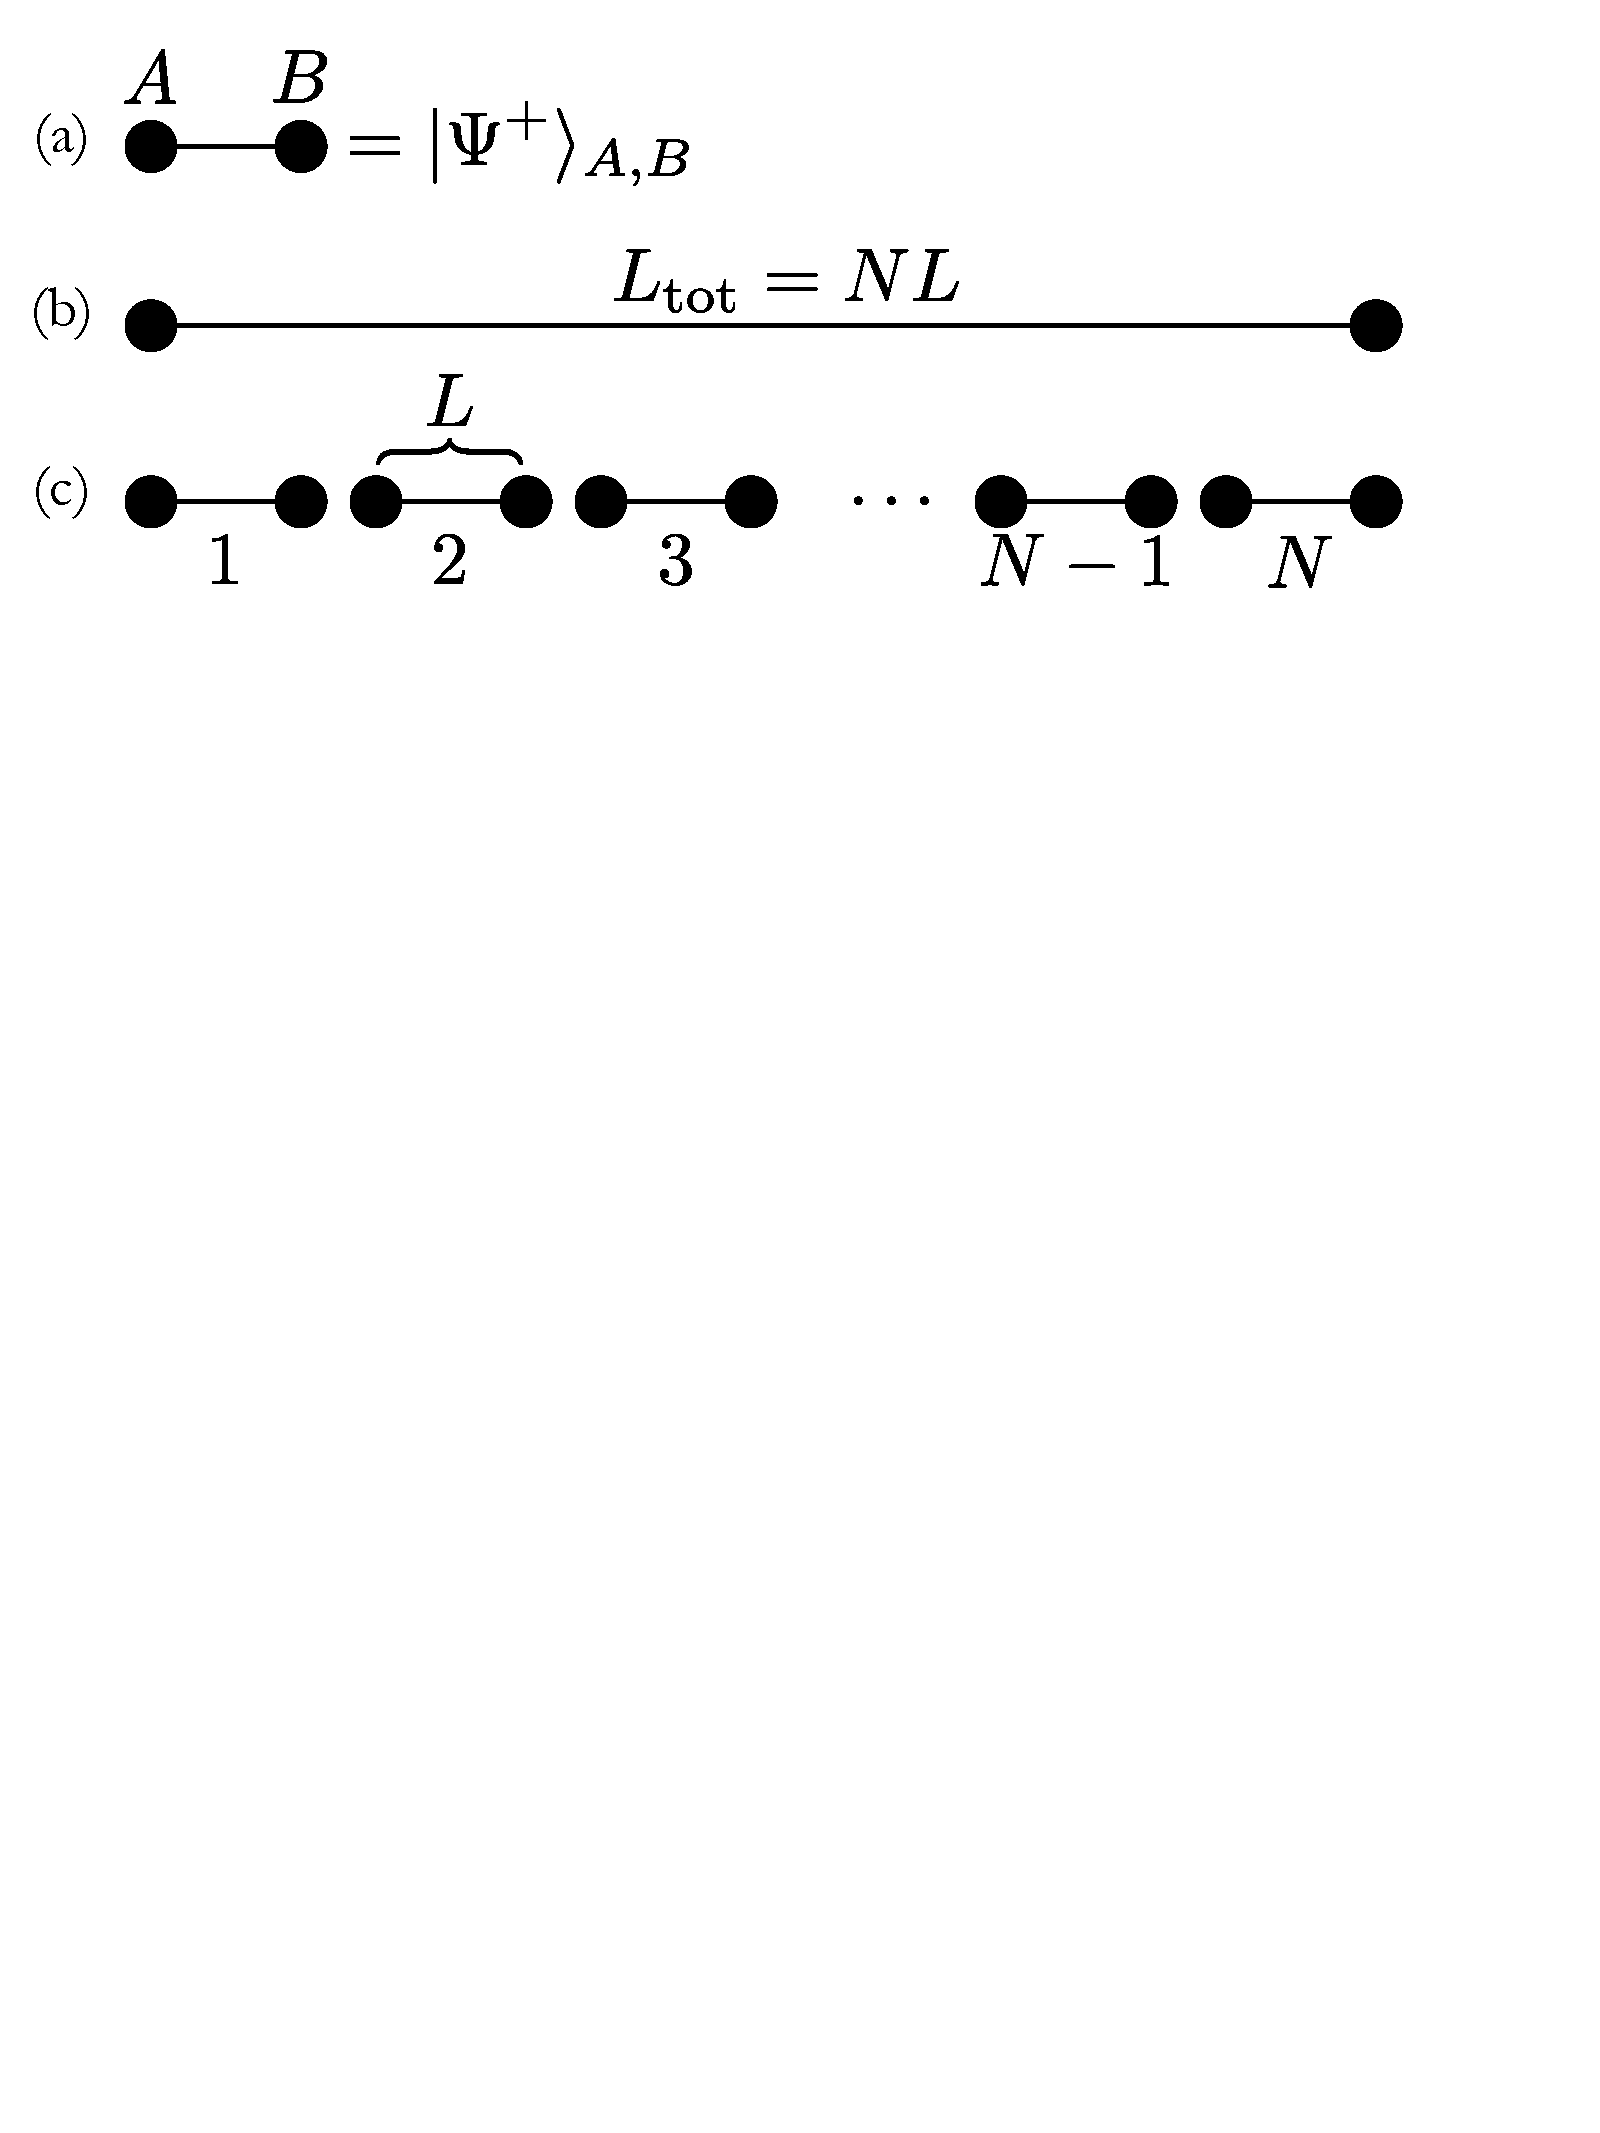
\includegraphics[width=0.475\textwidth]{repeaters_1}
\caption{(a) Schematic representation of an entangled Bell pair $| \Psi\rangle_{A,B}$ shared between remote parties Alice and Bob. The two solid dots represent physical qubits, while the edge represents entanglement. (b) The link may be over a long distance $L_{\rm tot}$. (c) Due to channel losses the link may be broken into $N$ smaller segments of length $L$. The links for each of the smaller segments can be independently generated and combined to form the longer distance link.} 
\label{fig:repeaters_1}
\end{figure} 

The links are now over much shorter distances and so can be generated with far higher probability \cite{}. Then by stitching these together using entanglement swapping (Sec.~\ref{sec:ent_swap})\index{Entanglement swapping}, we can generate our required long-range entanglement link \cite{}.

Beginning from this simple principle, the field of quantum repeater networks has grown enormously, leading to several generations of repeater designs, of ever increasing power and sophistication, and ever increasing technological demands.

\subsection{First generation repeaters}\index{First generation repeaters}

The above description is very hand-wavy, and of course things are a little more complicated in practise. We now examine these ideas in a little more detail, starting with a simple linear chain of repeater stations. 

In a quantum repeater network, there are three main operations required \cite{}:
\begin{enumerate}
\item Entanglement distribution (Sec.~\ref{sec:reps_ent_dist}): to create entangled links between adjacent repeater nodes \cite{}.
\item Entanglement purification (Sec.~\ref{sec:reps_ent_purif}): to improve the quality of entanglement between nodes \cite{}\index{Entanglement purification}.
\item Entanglement swapping (Sec.~\ref{sec:reps_ent_swap}): to join adjacent entangled links together to form longer distance links \cite{}\index{Entanglement swapping}.
\end{enumerate}
The basic operation of a repeater, as shown in Fig.~\ref{fig:repeaters_2}, works as follows:

We begin our preparation of a long-range entangled link by creating multiple entangled pairs between adjacent repeater nodes (the number will depend both on the quality of the pairs we initially generate and also the target quality we want our final pair to have). Once we have enough pairs established between two repeater nodes, we perform entanglement purification\index{Entanglement purification}, which converts multiple entangled links (pairs) into a fewer number with higher quality. 
\begin{figure}[!htb]
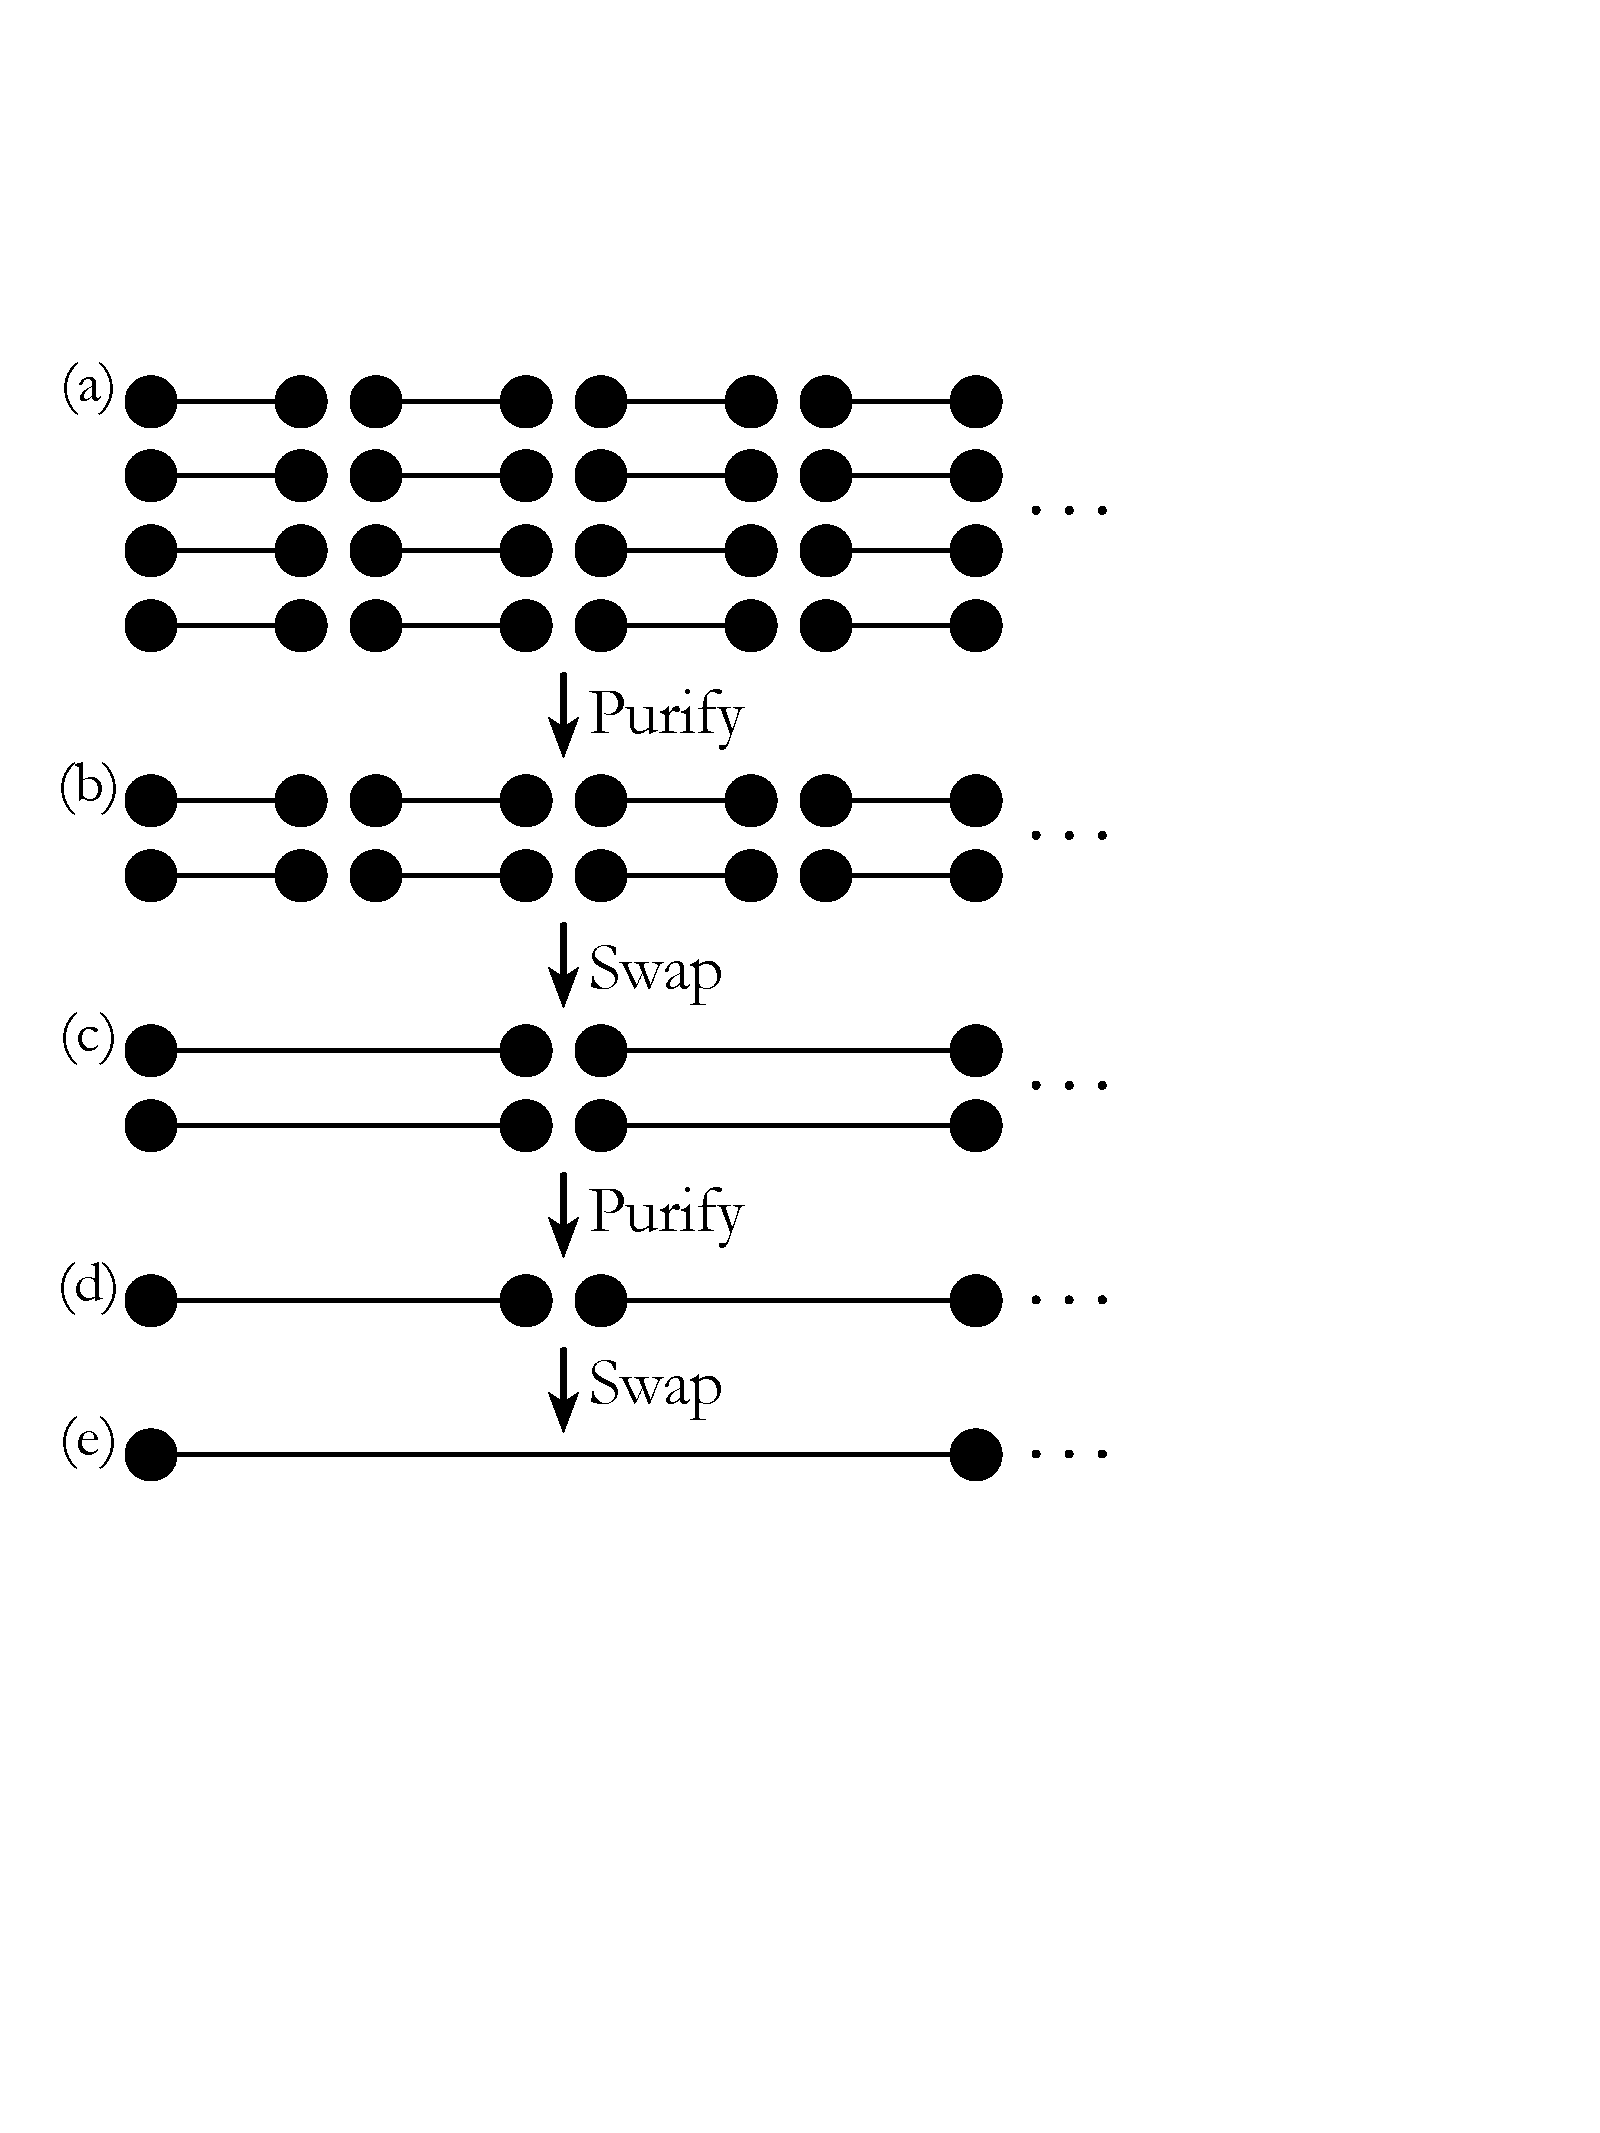
\includegraphics[width=0.4\textwidth]{repeaters_2}
\caption{Basic operation of a (first generation) quantum repeater network. (a) Preparation of multiple entangled links between adjacent repeater nodes. (b) They are then purified to create higher fidelity links. (c) Entanglement swapping between adjacent pairs creates links of twice the original length. (d) These new links are purified to create higher fidelity ones. (e) Entanglement swapping in creates a link four times the original size. This process continues as necessary to reach target distance and purity.} 
\label{fig:repeaters_2}
\end{figure} 
These purification steps, shown in Fig.~\ref{fig:repeaters_2}(a-b), are performed on the links between all adjacent repeaters, increasing the quality of the links between those adjacent repeater stations to the required degree. Entanglement swapping, as shown in Fig.~\ref{fig:repeaters_2}(c), then creates links twice as long. The resulting entanglement links can then be used for further rounds of purification and swapping until one generates a high quality link between the desired points in the network \cite{}. 

\subsubsection{Entanglement distribution}\index{Entanglement distribution}\label{sec:reps_ent_dist}

Probably the most important operation for any quantum repeater setup is entanglement distribution, the process of creating entanglement between two remote parties (Alice and Bob) connected by a quantum channel (generally an optical fibre or free-space link). This can be implemented in a number of ways \cite{bib:Bennett96, bib:nk98, bib:bennett93, bib:SSRG09, bib:childress06, bib:loock06, bib:munro08}, but can be broadly categorised into three basic schemas:
\begin{itemize}
\item Photon emission from quantum memories in the repeater nodes, followed by which-path erasure.\index{Which-path erasure}
\item Absorption of entangled photons by quantum memories.
\item Photon emission at one node and absorption at another.
\end{itemize}
By far, the emission based schemes are the most common, which we concentrate on here. Such schemes operate by using an entanglement process -- \textit{which-path erasure} -- to entangle two quantum memories via photons to which they were coupled.

We now describe such a which-path entangling operation in the context of 2-level quantum memories coupled to polarisation-encoded photons. A closely related scheme for preparing cluster states on $\lambda$-configuration systems for the purposes of quantum computation is discussed in Sec.~\ref{sec:barrettkok_lambda}.

Ideally one wants to generate a maximally entangled state of the form \cite{bib:WJM2015},
\begin{align}
|\Psi\rangle=\frac{1}{\sqrt{2}} (|g\rangle |H\rangle + |e\rangle |V\rangle),
\end{align}
within the repeater node, where $\ket{g}$ and $\ket{e}$ are the two states (ground and excited) of the quantum memory, and $\ket{H}$ and $\ket{V}$ are the polarisation states of light. 
\begin{figure}[!htb]
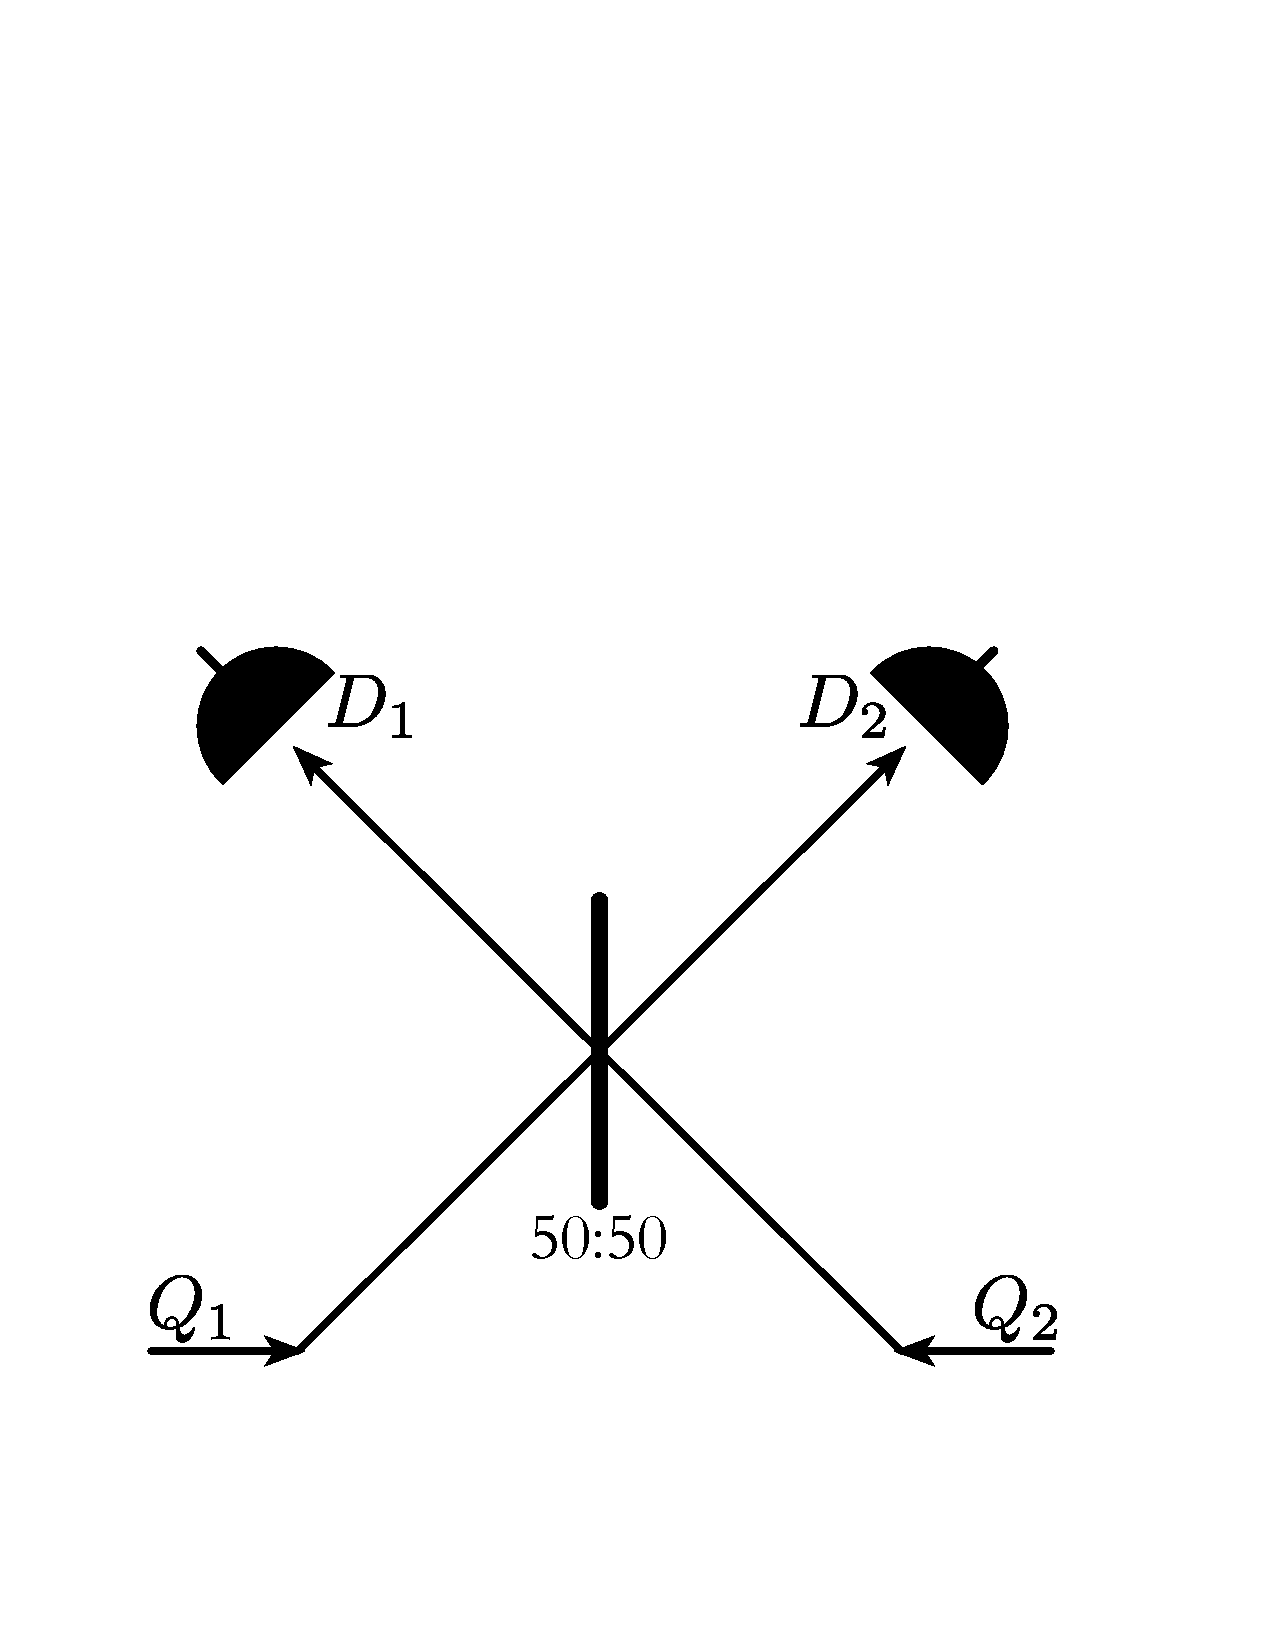
\includegraphics[width=0.3\textwidth]{repeaters_3}
\caption{Entanglement distribution scheme based on quantum emitters and which-path erasure\index{Which-path erasure}. Each node emits a photon entangled with the quantum memories present within that nodes. The photons from the adjacent repeater nodes then interfere on a beamsplitter (or polarising beamsplitter)\index{Beamsplitter}\index{Polarising beamsplitter} which erases information about which path the photon took. The photons are then measured in an appropriate basis to project the quantum memories within the nodes onto an entangled state.} 
\label{fig:repeaters_3}
\end{figure} 
The photons from the two repeater nodes (Fig.~\ref{fig:repeaters_3}) are then transmitted to a beamsplitter (or PBS in this example), after which the state of the system is,
\begin{align}
|\Psi\rangle &= \frac{1}{2} |g\rangle |g\rangle |H\rangle |H\rangle +\frac{1}{2} |e\rangle |e\rangle |V\rangle |V\rangle \nonumber \\
&+\frac{1}{2} |g\rangle |e\rangle |HV\rangle |0\rangle + \frac{1}{2} |e\rangle |g\rangle |0\rangle |HV\rangle. 
\end{align}

One immediately notices that the $|g\rangle |e\rangle$ and $|e\rangle |g\rangle$ contributions are associated with two photons in one of the PBS exit modes, the other being in the vacuum state. However, the $|g\rangle |g\rangle$ and $|e\rangle |e\rangle$ terms have one photon in each of the output modes. They are of opposite polarisation, but measuring those photons in the diagonal/anti-diagonal ($\hat{X}$) basis erases this `which-path' information yielding an equal superposition of the two alternative histories -- an entangled state of the form,
\begin{align}
|\Psi_\pm\rangle=\frac{1}{\sqrt{2}} (|g\rangle |g\rangle \pm |e\rangle |e\rangle),
\end{align}
where the sign is given by the parity of the two photo-detection outcomes in the $\hat{X}$ basis. This entangled state is stored in the quantum memories between nodes \cite{}. 

The scheme based on photon absorption by the quantum memories is effectively the time reversal of the emission-based scheme \cite{}. Instead of using the beamsplitter to entangle the photons emitted from each memory, a source of entangled photon(s) is employed \cite{}. Of course, the emission and absorption schemes can be used together in a hybrid architecture.

In any entanglement distribution scheme for quantum networks, the repeater nodes are spatially separated and one must consider channel losses, which are the dominant error source. Channel loss in this situation implies that we do not register a coincidence event between $D_1$ and $D_2$, which heralds the entanglement. Thus our entanglement distribution success probability is reduced. In fact, the heralded probability of success can be expressed as \cite{},
\begin{align}
p_\mathrm{ED}= \frac{1}{2} e^{-L/L_0} {p_\mathrm{det}}^2,
\end{align} 
where $L$ is the distance between the two repeater nodes with $L_0$ being the attenuation length of the channel, while $p_\mathrm{det}$ is the detector efficiency. Here we have ignored the source and coupling efficiencies. It is immediately obvious from this expression that the further the repeater nodes are apart, the lower the probability of success, on an exponentially decaying trajectory. The attenuation length of typical telecom optical fibre is approximately 22.5km and so the average time to generate a distributed entangled pair is,
\begin{align}
T_\mathrm{av} &\sim \frac{L}{ c \cdot p_\mathrm{ED}}\nonumber\\
&= \frac{2 L e^{L/L_0}}{ c \cdot {p_\mathrm{det}}^2}
\end{align} 
where $c$ is the speed of light in the channel. This grows exponentially against node separation and so places important constraints on the lifetime of the quantum memories. If we consider pure dephasing effects on our matter qubits, the state of our system can be represented by,
\begin{align}
\hat\rho(F) = F |\Psi^+\rangle \langle \Psi^+|+(1-F) |\Psi^-\rangle \langle \Psi^-|,
\label{eq:rho_bell_fid}
\end{align} 
where $F$ is the fidelity of our entangled state given by,
\begin{align}
F=\frac{1+e^{-t/\tau_\mathrm{D}}}{2},
\end{align} 
with $t$ being the duration over which the entangled state is held in memory, while $\tau_\mathrm{D}$ is the coherence time of the memory. If one only requires a single Bell pair and no further operation are performed, then \mbox{$t=c/L$}. However in a more general setting where multiple pairs are required, the time will be $T_\mathrm{av}$ on average, which is inversely proportional to the probability of generating the entangled state. The quality of the prepared remote entangled state may therefore not be sufficient for the tasks it is required for due to these finite memory lifetimes or operational gate errors. One needs to be able to purify these entangled resources. 

\subsubsection{Entanglement purification}\index{Entanglement purification}\label{sec:reps_ent_purif}

The finite coherence-time of quantum memories and operational errors caused by quantum gates means some mechanism will be required to improve the fidelity of the distributed entangled state, especially if the spatial separation is large. This is generally achieved by entanglement purification \cite{bib:Bennett96, bib:Deutsch98, bib:dur98, bib:pan01, bib:dur07, bib:Aschauer2004, bib:jiang09, bib:munro12, bib:Stephens2013} which  as it name implies purifies the entanglement to a higher value. The purification operation uses either an error detection code (probabilistic but heralded operations) \cite{bib:Bennett96, bib:Deutsch98, bib:dur98} or deterministic error correction codes \cite{bib:Aschauer2004, bib:jiang09, bib:munro12}. While the error correction codes purify in a deterministic way, they place tough constraints on both the required initial fidelity of entangled states and also the quality of the quantum gates implementing the purification \cite{bib:Aschauer2004}. Given this, we will focus on the simplest error detection code which requires only a pair of shared entangled quantum memories (as shown in Fig.~\ref{fig:repeaters_4}). This scheme is equivalent to the entanglement purification protocol described in Sec.~\ref{sec:ent_purif}, although the graphical notation is somewhat different.

\begin{figure}[!htb]
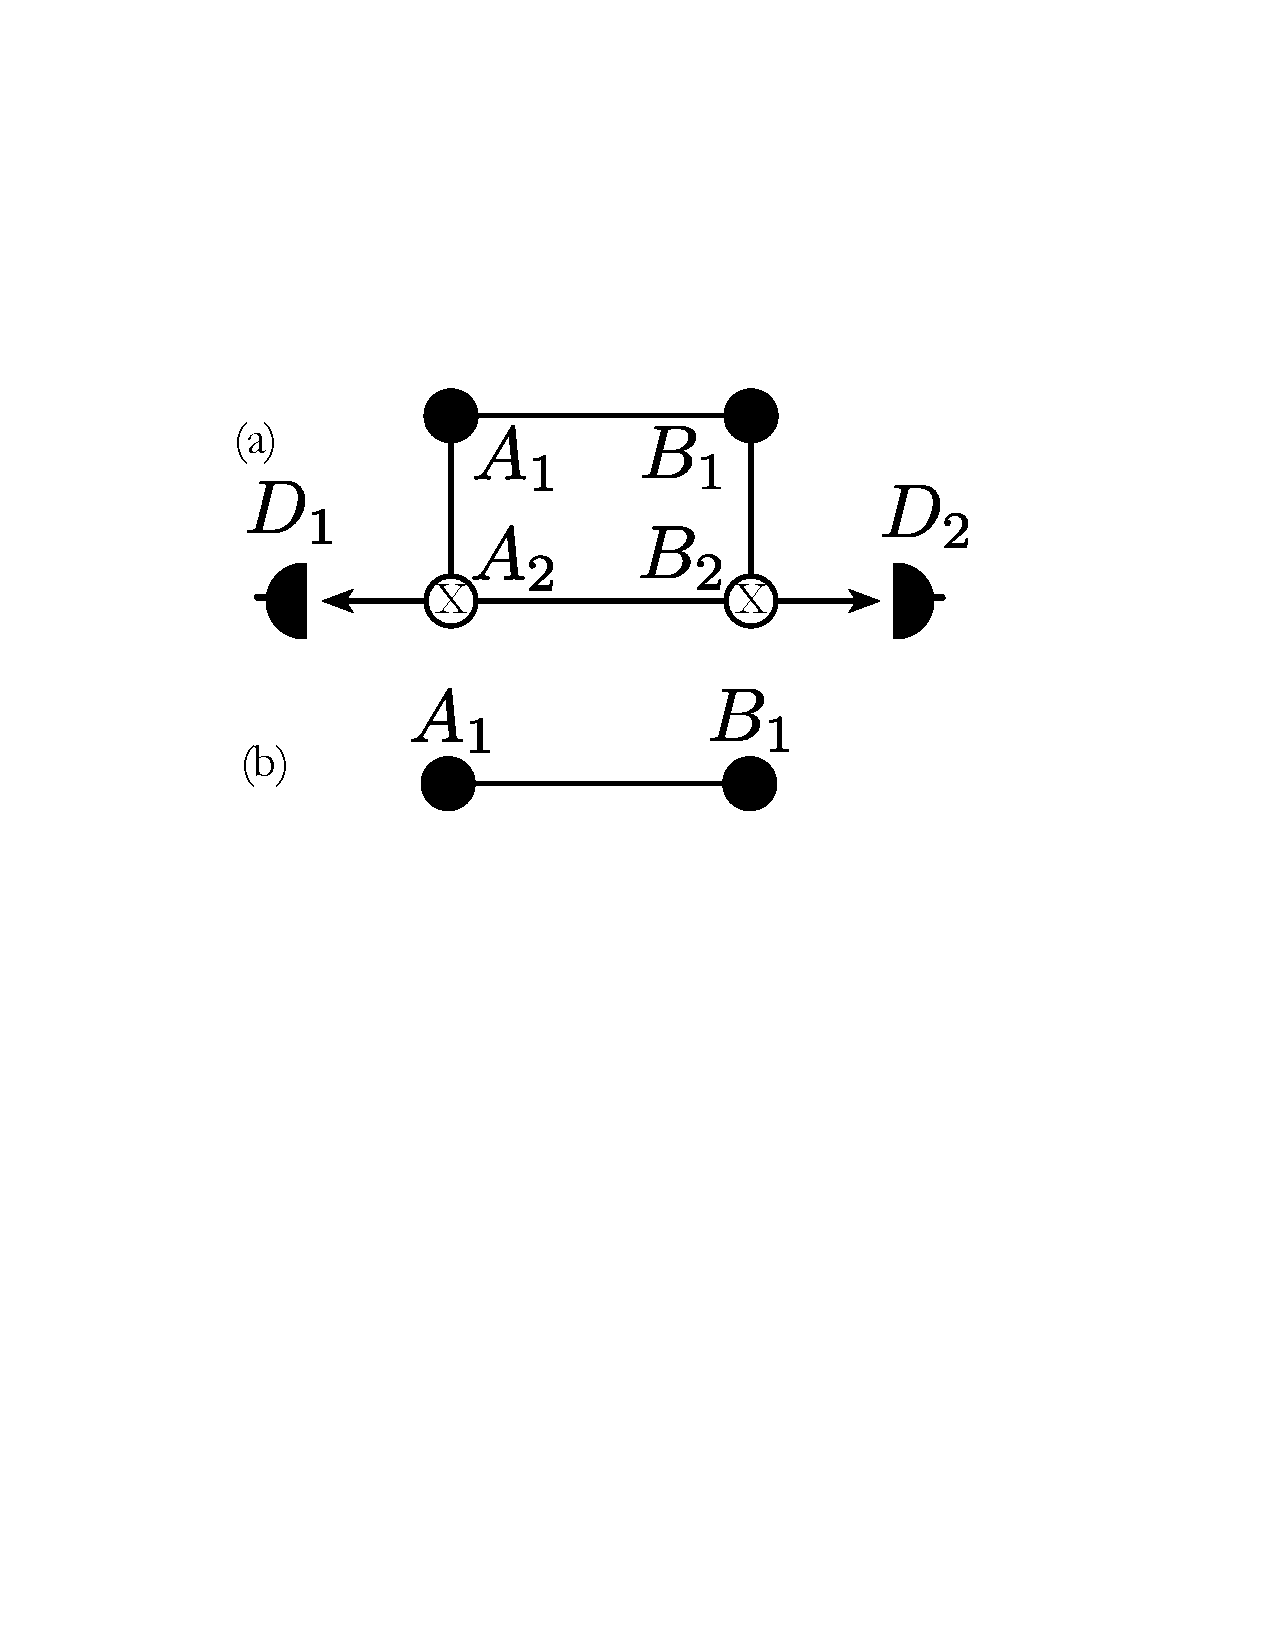
\includegraphics[width=0.35\textwidth]{repeaters_4}
\caption{Entanglement purification: (a) The simplest purification scheme involving two pairs of shared remote entangled quantum memories (\mbox{$A_1-B_1$} and \mbox{$A_2-B_2$}). The purification operation begins with Alice performing a CNOT operation between memories $A_1$ and $B_1$. Similarly Bob performs a CNOT operation between his memories. Alice and Bob then measure qubits $A_2$ and $B_2$ in the computational ($0$, $1$) basis and share their results. They discard the resulting state if between them they measured odd parity ($0,1$ or $1,0$). They keep the state if they measured an even parity between them ($0,0$ or $1,1$) which should have higher fidelity. (b) Two qubits are removed, leaving a residual two-qubit state between $A_1$ and $B_1$ with improved fidelity.} 
\label{fig:repeaters_4}
\end{figure} 

In this simplest purification protocol, Alice and Bob share two pairs of entangled states of the form given by Eq.~(\ref{eq:rho_bell_fid}). These states are a mixture of only two Bell states. We begin our purification protocol by using local operations to transform $\hat\rho$ to,
\begin{align}\label{eq:rho_bell_fid_dash}
\hat\rho(F)=F |\Psi^+\rangle \langle \Psi^+|+(1-F) |\Phi^+\rangle \langle \Phi^+|,
\end{align}

As shown in Fig.~\ref{fig:repeaters_4} we then apply a CNOT gate between Alice's two memories and Bob's two memories following by measuring $A_2,B_2$ in the computational basis. Upon measurement of even parity our resulting state $\hat\rho(F')$ has the form, but with new fidelity,
\begin{align}
	F'=\frac{F^2}{F^2+(1-F)^2}.
\end{align}

It is immediately obvious that our resulting state $\hat\rho(F')$ is more entangled that $\hat\rho(F)$ when \mbox{$F>1/2$} (see Fig.~\ref{fig:rep_purification}). In fact the degree of entanglement as measured by the concurrence\index{Concurrence} increases from,
\begin{align}
	C=2 F-1,
\end{align}
to,
\begin{align}
C' &=2 F'-1 \nonumber\\
&= \frac{2 F^2}{F^2+(1-F)^2}-1.
\end{align}

\begin{figure}[!htb]
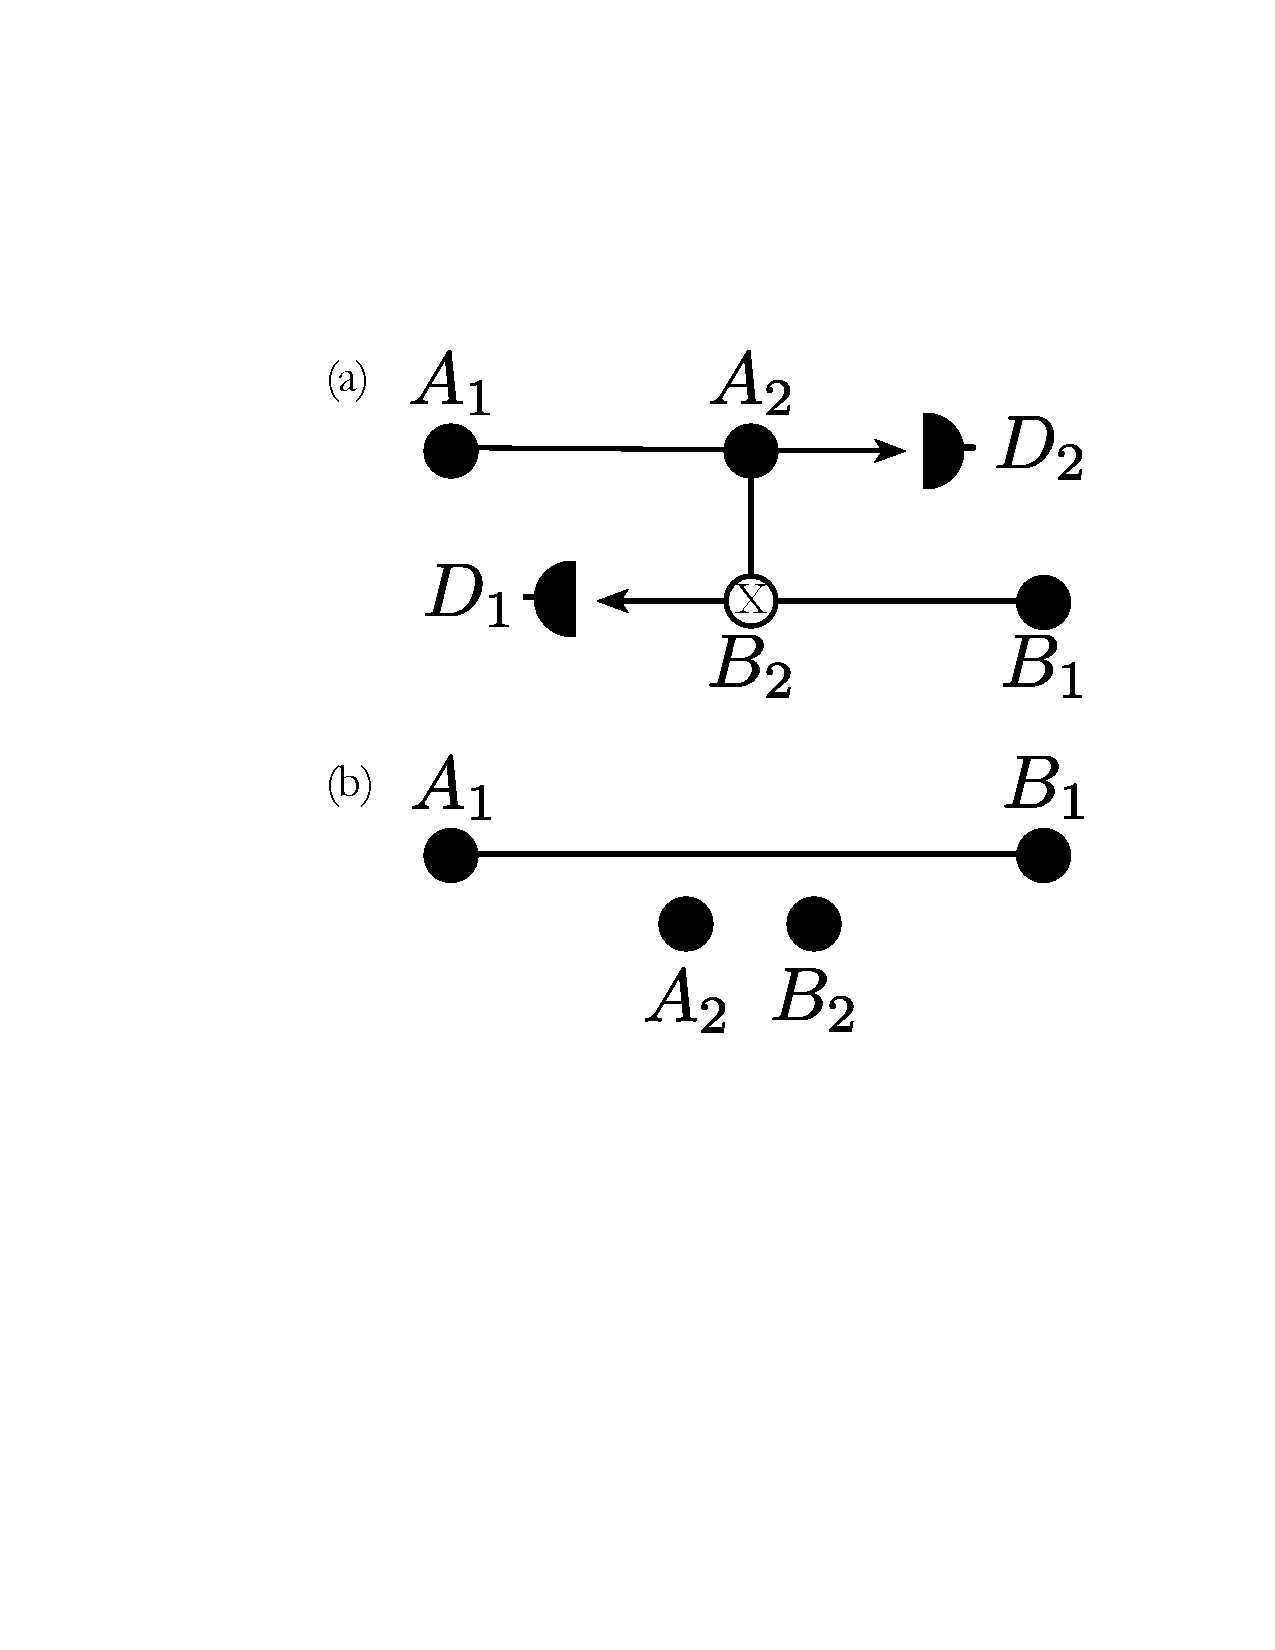
\includegraphics[width=0.35\textwidth]{repeaters_5}
\caption{Plot of the increased fidelity and success probability for entanglement purification for a mixture of two Bell states with initial fidelity $F$. The dashed lines show how multiple pairs with an initial fidelity $F=0.7$ can be purified iteratively to a final fidelity above 0.95.} 
\label{fig:rep_purification}
\end{figure} 

It is important to mention that the entanglement purification doesn't allow one to distribute a \textit{perfect} Bell state. Rather it \textit{asymptotically} approaches perfection (under ideal conditions) with repetition of the protocol.

The probability of obtaining the even parity outcome is,
\begin{align}
	p_\mathrm{even}=\frac{F^2+(1-F)^2}{2}.
\end{align}
Alternatively for the odd parity measurement results, which occur with probability,
\begin{align}
	p_\mathrm{odd}=F(1-F),
\end{align}
the resulting state is an equal mixture of $|\Psi^+\rangle$ and $|\Phi^+\rangle$ and is not entangled at all. In this case we must start again from scratch with the entanglement distribution.

So far we have discussed one round of entanglement purification but the protocol naturally works in a recursive way where two copies of a state with the same fidelity are used for the next purification round. Using this bootstrapped approach one can in principle generate a near unit fidelity entangled pair from a finite fidelity pair (provided initial input fidelity \mbox{$F>1/2$}). 

There are two common variants of these purification protocols: the Deutsch and Dur variants:
\begin{itemize}
\item \textit{Deutsch protocol} \cite{bib:Deutsch98}: This is an efficient purification protocol utilising Bell diagonal states that reaches a high fidelity in a few purification rounds. It is assumed that both entangled pairs have the same form. The purification protocol is the same at the one described above in Fig.~\ref{fig:repeaters_4}, but begins with Alice (Bob) applying $\pi/2$ $(-\pi/2)$ rotations about the $X$-axis on their qubits before the usual CNOT gates and measurements are performed. Two copies of the successfully purified pair can then be used in a recursive approach to purify either further. This in turns means multiple copies of the originally distributed states are required. We must have enough entangled pairs available to perform the multiple rounds of purification that are required, which grows exponentially with the number of purification rounds. 

\item \textit{Dur protocol} \cite{bib:dur98}: This uses the same core purification elements shown in Fig.~\ref{fig:repeaters_4} but relaxes the traditional constraint that both Bell pairs must have the same fidelity. Instead we begin with two pairs of the same fidelity $F$, and perform the traditional purification. If successful we perform the next round of purification using the improved fidelity pair from the previous round and a fresh fidelity $F$ pair. In effect this new auxiliary pair is used to boost the fidelity of the original pair higher. This can continue until we reach a limiting fidelity dependent on the original $F$. This limiting fidelity may be above the desired resultant fidelity, at which point we can terminate the purification protocol. A significant difference between the Deutsch and Dur protocols is that the number of memories in the Dur situation is linear in the number of nesting levels.
\end{itemize}

It is critical in repeater protocols to also discuss how fast these purification protocols can be performed. Even with ideal gates one has to wait for the parity information to be shared between the repeater nodes. For nodes separated by a distance $L$, the communication time for a single trial is $L/c$. However, remembering that purification is probabilistic but heralded in nature our waiting time could be many multiples of $L/c$. This will have a dramatic effect on performance, especially if performed at many different stages in the network with increasing distances between nodes.

\subsubsection{Entanglement swapping}\label{sec:reps_ent_swap}\index{Entanglement swapping}

The entanglement distribution and purification scheme discussed previously allow one in principle to create high fidelity entangled states between adjacent repeaters nodes. The next task is to extend the range of our entangled states, and this occurs via simple entanglement swapping \cite{bib:BDCZ98, bib:Zukowski93, bib:goebel08, bib:duan01}. This was described previously in Sec.~\ref{sec:ent_swap}, although the notation is modified.

\begin{figure}[!htb]
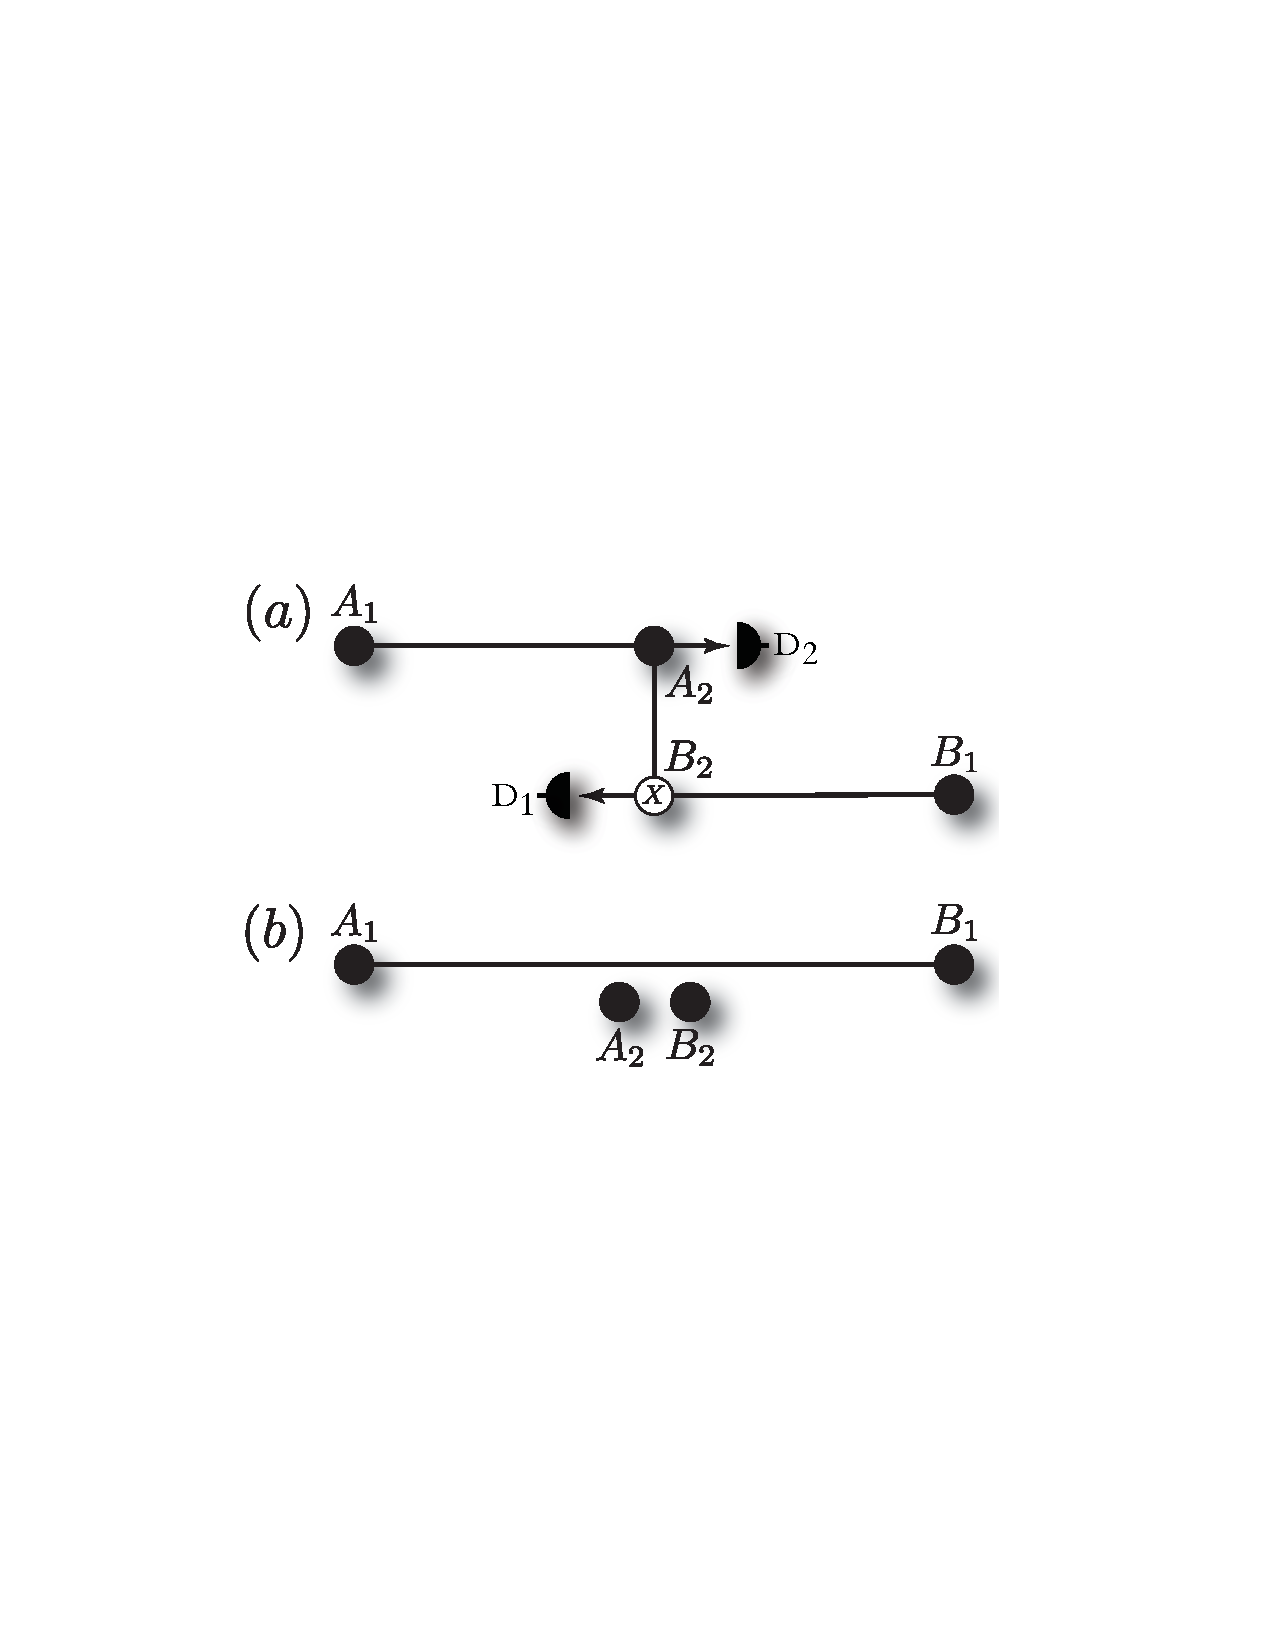
\includegraphics[width=0.4\textwidth]{repeaters_6}
\caption{Entanglement swapping: (a) An entangled state is shared between Alice and a repeater station ($A_1-A_2$), and also between the repeater station and Bob ($B_2-B_1$). The entanglement operation begins by performing a Bell state measurement between $A_2$ and $B_2$ using a CNOT gate, and measurements at $D_1$, $D_2$.  The measurements indicate which Bell state we have projected our state $A_1$, $B_1$ onto. (b) The resultant entangled state between $A_1$, $B_1$ with the qubits $A_2$ and $B_2$ disentangled from it.}
\label{fig:repeaters_6}
\end{figure} 

Consider the situation where we have an entangled Bell pairs between nodes $A_1$ and $A_2$ and also between $B_2$ and $B_1$. The entanglement swapping operation involves a Bell state measurement between the qubits $A_2$ and $B_2$ as shown in Fig.~\ref{fig:repeaters_6}. After the Bell measurement we have the resultant state, 
\begin{align}
\hat\rho_{A_1,A_2} (F)\otimes \hat\rho_{B_2,B_1}(F)\rightarrow \hat\rho_{A_1,B_1} (F')
\end{align}
with,
\begin{align}
	F'=F^2+(1-F)^2,
\end{align}
where a local correction operation is performed on either $A_1$ or $B_1$ depending on the measurement outcome. It is clear that the longer range entangled state $\hat\rho_{F'}$ is less entangled that the states $\hat\rho_F$ used to generate it. In fact, to first order our fidelity drops from $F$ to $F^2$. This in turn means that we can not simply purify adjacent repeater pairs and swap them all to create the long range pairs. If we had $n$ links, our final fidelity from all the swapping would scale as $F^n$. For high fidelity end-to-end entangled links we need to follow the approach outlined in Fig.~\ref{fig:repeaters_2}. Finally, depending on how the Bell measurement is implemented, this process could be probabilistic (but heralded) or deterministic in nature. We assign the success probability as $p_\mathrm{ES}$.

\subsubsection{Performance}\index{Repeater performance}

We now have all the operations required for a repeater to create long-range entanglement. The natural question to ask is how well it performs.

There are several important points to initially consider here. The majority of the repeater operations are probabilistic in nature (entanglement distribution and purification fundamentally, and entanglement swapping dependent upon implementation). While these probabilistic operations may be heralded, classical signalling must be performed between involved nodes  to inform them of successes or failures. For entanglement distribution this time is just that associated with the signalling between adjacent nodes. However, purification and swapping are likely to require such signalling over the entire length of the network. This has a dramatic effect on the performance of the repeater network. The normalised rate for generating Bell-pairs over a total distance $L_\mathrm{tot}$ is given by,
\begin{align}
R(n,k,L_\mathrm{tot})= \frac{1}{T_{n,k,L_\mathrm{tot}} M_{n,k}}
\label{eq:rep_net_resources}
\end{align}
where $T_{n,k,L_\mathrm{tot}}$ is the time to generate a Bell-pair over the total distance using an $n$-nested repeater configuration with $k$ rounds of purification per nesting level. The distance between repeater nodes is given by,
\begin{align}
	L=\frac{L_\mathrm{tot}}{2^n},
\end{align}
meaning there are \mbox{$2^n-1$} intermediate repeater nodes with Alice and Bob at the endpoints. In Eq.~(\ref{eq:rep_net_resources}) we discount our rate by $M_{n,k}$, the total number of quantum memories used. The justification for this is that this provides a fairer comparison when different purification approaches are used. The Deutsch protocol for instance achieves its target fidelity much faster (fewer rounds) than the Dur protocol, but consumes far more resources in doing so. \comment{Did I correct this paragraph correctly?}

Now it is straightforward, albeit tedious, to show that $T_{n,k,L_\mathrm{tot}}$ is given by \cite{bib:braztzik2013},
\begin{widetext}
\begin{align*}
 T_{n,k,L_\mathrm{tot}} &\sim \frac{3^n}{2^{n-1} p_\mathrm{ED}} \prod_{i=0}^{n-1} \left(\frac{3}{2}\right)^{k}  \frac{1}{P_\mathrm{ES}(n-i)  }\prod_{j=0}^{k-1} \frac{1}{p_\mathrm{P}(k-j,n-i)}  \nonumber \\
 &+\sum_{m=1}^n\left(\frac{3^{n-m}}{2^{n-1}}\right) \prod_{i=0}^{n-m}   \left(\frac{3}{2}\right)^{k} \frac{1}{P_\mathrm{ES}(n-i)}  \prod_{j=0}^{k-1}  \frac{1}{p_\mathrm{P}(k-j,n-i)}  \\
&+\sum_{m=1}^n {\sum_{q=0}^{k-1} \left(\frac{3^{n-m+q}}{2^{n- 2 m+q}}\right) \prod_{r=0}^{q}\frac{1}{p_\mathrm{P}(k-r,m)}} 
\prod_{i=0}^{n-m-1}   \left(\frac{3}{2}\right)^{k} \frac{1}{P_\mathrm{ES}(n-i)}  \prod_{j=0}^{k-1}  \frac{1}{p_\mathrm{P}(k-j,n-i)} \nonumber 
\end{align*}
\end{widetext}
where $p_\mathrm{ED}$ is the probability of successfully distributing entanglement between adjacent repeater nodes, while $p_\mathrm{P}(j,i)$ [$p_\mathrm{ES}(i)$] represents the purification [entanglement swapping] probability at the $i$th nesting level with $j$ rounds of purification. The factors of $3/2$ present in all entanglement distribution, purification and swapping operations is a multiplicative factor associated with the extra time required for the two pairs to be available for the various quantum operations \cite{bib:SSRG09}.

It can be easily seen from this formula that,
\begin{align}
	T_{n,k,L_\mathrm{tot}} \gg \frac{2 L_\mathrm{tot}}{c},
\end{align}
especially if probabilistic gates are included. Next the resources scale polynomially with,
\begin{align}
	M_{n,k} &\sim 2^{(k+1)n}\nonumber\\
	&\sim \left(\frac{L_\mathrm{tot}}{L}\right)^{k+1},
\end{align}
for the Deutsch protocol, which in turn implies it is efficient. However for long distances $L_\mathrm{tot}$, our normalised rate \mbox{$R(n,k,L_\mathrm{tot})\ll 1\mathrm{Hz}$}, especially when probabilistic CNOT gates and Bell state measurements are employed \cite{bib:jiang09, munro10}.

\subsection{Second generation repeaters and error correction}\index{Second generation repeaters}

The previous approach for entanglement distribution over long distances based on first generation quantum repeaters has its performance heavily constrained by both the probabilistic nature of the various quantum operations and the associated classical communication time. We know that the classical communication in entanglement distribution is only between the adjacent nodes, whereas for the purification and swapping operations it can be very long-range, potentially over the entire network length. This is the fundamental reason why the time to create a pair is of order $O(L_\mathrm{tot}/c)$ or longer. This will not change significantly even if we have deterministic CNOT gates and Bell measurements as the entanglement purification protocols will remain probabilistic in nature (even though the swapping operations will be deterministic). We thus need to replace our usual entanglement purification protocols with a similar operation that is deterministic in nature \cite{bib:jiang09, bib:munro10}.

The typical entanglement purification protocols are a form of quantum error detection code \cite{bib:WJM2015, bib:devitt2013} (see Sec.~\ref{sec:QOS} for further discussion on quantum error detection and correction). Such codes herald whether an error has occurred or not, and in the situation considered above, detection of errors means one must discard the entangled pairs associated with the purification protocol. No errors means the purification protocol has worked.

Error correction codes which operate in a deterministic fashion can also detect errors and can be used in this fashion \cite{bib:jiang09, bib:munro10}. More critically, quantum error correction codes have the potential to correct some errors that have occurred, mitigating the need to completely discard states affected by errors. For normal error correction protocols used in quantum computations, we encode our physical qubits into logical qubits using the code, and then use syndrome measurements to determine where an error has potentially occurred.

Quantum communication however is different in this case as we must assume we have generated a number of imperfect Bell pairs between the repeater nodes before we utilise the error correction schemes. The error correction protocol in this case operates by using the error correction encoding circuit on Alice's qubits and the decoding circuit on Bob's \cite{bib:Aschauer2004} as illustrated in Fig.~\ref{fig:repeaters_7} for the 5-qubit code\index{5-qubit code} \cite{bib:Bennettr1996a, bib:Knill97}.

\begin{figure*}[!htb]
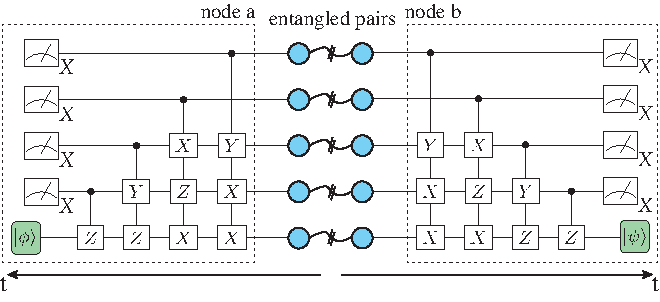
\includegraphics[width=\textwidth]{repeaters_7}
\caption{\comment{Redo fig} Schematic illustration of a purification circuit based on quantum error correction. The specific example shown is for the [[5,1,3]] code \cite{bib:Bennettr1996a, bib:Knill97}. We assume that entanglement distribution has allowed Alice and Bob to create 5 copies of their imperfect Bell pairs. The error correction circuit is executed independently between the two nodes. While we show the situation when the measurements at both sides are done directly on four pairs of entangled qubits (leaving us with one unencoded Bell pair), one can also use ancilla qubits to measure the appropriate syndromes. As soon as the measurements are complete both nodes' qubits are available for continued use as the error correction is deterministic and there are no failure events that need to be heralded. In this case the classical message between nodes just carries Alice's measurement results, allowing either node to interpret which Bell state was generated and for one of them to apply the bit-flip or phase-flip correction operation if needed to recover the desired Bell state. In many cases this correction is classically tracked in the Pauli frame (the Pauli frame indicates whether an $\hat{X}$, $\hat{Z}$ or both need to be performed at some stage \cite{bib:jiang09, bib:munro10}). Note that it's not necessary to measure out all but one of the qubits involved in the entangled links. Instead the logical qubit can be maintained by the use of ancilla qubits within that node with the syndrome being measured with the help of the ancilla qubits. Entanglement swapping could then be performed on the logical qubits enabling a much more error resilient system.
}
\label{fig:repeaters_7}
\end{figure*} 

It's important to state here that error correction-based purification is deterministic in nature (there is however a significant cost that must be paid -- the fidelity of the originally generated entanglement between adjacent nodes must be quite high) \cite{bib:jiang09, bib:Aschauer2004}. There are no measurement events that need to be discarded. Instead the measurement results only inform us of which particular imperfect Bell states we have and the correction operation required to return to the desired state. In effect the measurement is updating the Pauli reference frame\index{Pauli reference frame} \cite{bib:Knill2005}. This does not need to be executed immediately, and may be deferred until later. In turn this means once the measurements have been performed, we can immediately use the purified Bell state without having to wait for the classical signalling (at some stage the correction operation needs to be executed but this can be once the long distance entanglement has been generated). 

Mitigating having to wait for the measurement results to be sent and received in both the quantum error correction-based purification and entanglement swapping protocols has a profound effect on the rate of generating long-range entangled pairs. We still need to perform long-range classical messaging (potentially between end nodes), and thus it's immediately obvious that the preparation time can scale solely as,
\begin{align}
	T = \frac{2 L_\mathrm{tot}}{c},
\end{align}
which was the lower bound on the first generation schemes \cite{bib:munro10}.

Naively this seems to imply that the generation rate between end nodes cannot be faster than this. However, one can in fact do far better! This is shown in Fig.~\ref{fig:repeaters_8} (protocol described in caption). The key issue is that the generation rate depends on how long the adjacent nodes need to store part of an entangled state \cite{bib:jiang09, bib:munro10, bib:Muralidharan2016}. 

\begin{figure*}[!htb]
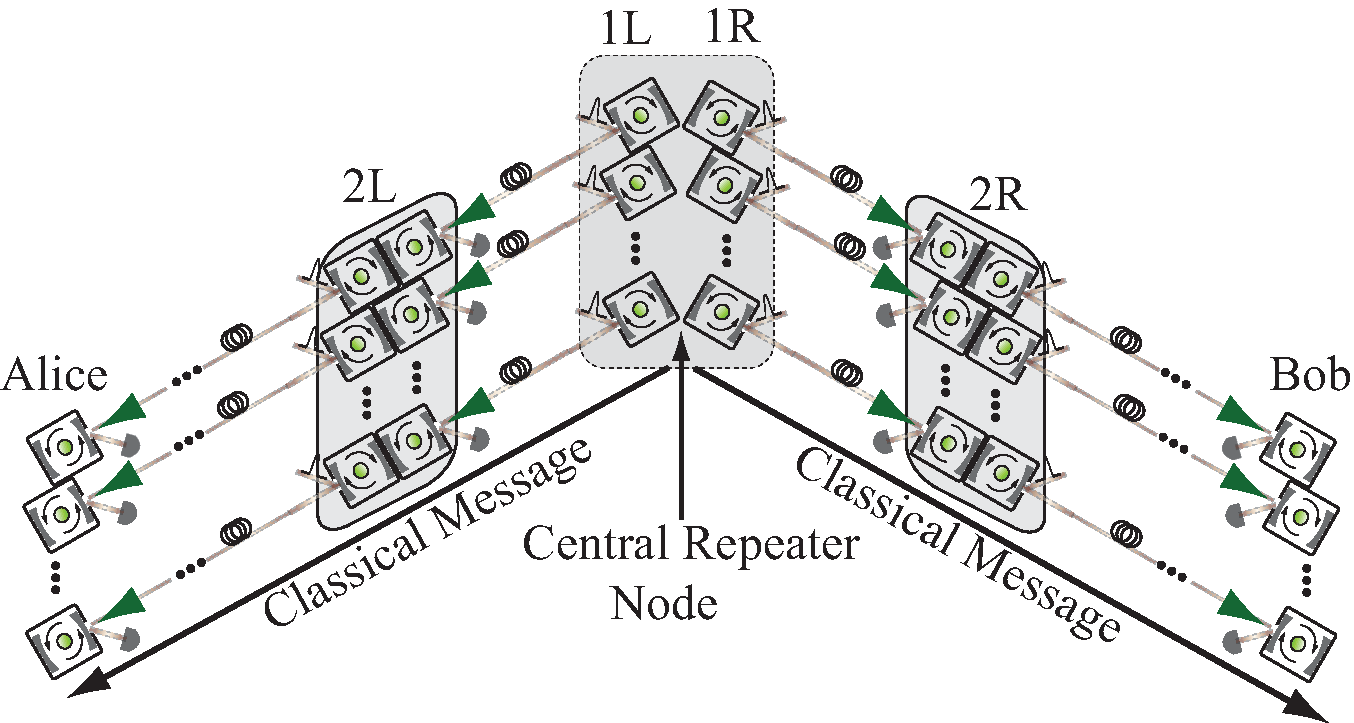
\includegraphics[width=\textwidth]{repeaters_8}
\caption{\comment{Redo fig}A butterfly design quantum repeater network protocol that reduces the requirements on all the quantum memory times to only that associated with the signalling time between adjacent repeater nodes \cite{bib:munro10}. Enough pairs must be generated between the node to ensure that we can use them in the error correction code in a single round trip time between adjacent nodes. The scheme relies on multiple entangled pairs being generated temporally, starting from the mid point of the network. The protocol begins with the central node creating links to both the left and right nearest neighbour nodes in sufficient number to allow an error correction code to be implemented. Once they are created the error correction circuits are applied to the links left and right of this central node (effectively creating encoded logical links). Entanglement swapping at the middle node is then applied  between these logical links, creating a logical link between the left and right adjacent nodes. The left and right nodes can then do the same to their next adjacent repeater nodes, error correcting as they go, until the desired end-to-end entangled link is achieved.  }
\label{fig:repeaters_8}
\end{figure*} 

Fundamentally we know that the time to attempt to generate a single entangled Bell pair between two nodes is scaling as $L/c$ (where $L$ is the distance between those two nodes). With channel losses we need to make,
\begin{align}
m=\frac{\log_{10} (\epsilon)}{\log_{10} (1-p_\mathrm{ED})} - \log_{10} (\epsilon / p_\mathrm{ED}),
\end{align}
attempts to generate a single Bell pair with error probability $\epsilon$. We can make these attempts simultaneously and not affect the generation time. Now by using a butterfly repeater design, as illustrated in Fig.~\ref{fig:repeaters_8}, one immediately notices that the qubits with the repeater nodes are only used for duration $\sim 2 L/c$. After this time those qubits have been freed up and are available to generate new entangled links. This means in turn that the time to generate the long-range entangled pair will scale as \mbox{$T\sim O(2L/c)$} (independent of the overall distance $L_\mathrm{tot}$) \cite{bib:jiang09, bib:munro10, bib:Muralidharan2016}. The exact resources used depends heavily on the error correcting code, but we know they in principe scale as \mbox{$M \sim O(\mathrm{polylog}(L_\mathrm{tot}))$} \cite{bib:Muralidharan2016}.

This is quite a dramatic decrease in both $T$ and $M$ compared to the first generation. In fact one could expect the normalised rates to be on the order of kHz \cite{bib:munro10}. However this is a significant cost in terms of the quality of the original Bell pairs that must be prepared. In the first generation schemes a fidelity just over 50\% was sufficient. However with the second generation schemes using normal error correcting codes, it is likely this initial fidelity will have to be over 90\% \cite{bib:jiang09, bib:munro10}. 

\comment{Up to here}

\subsection{Third generation repeaters}

The use of error correcting codes significantly improves the performance of second generation quantum repeaters compared to first generation ones. The second generation schemes are now limited by the communication time between adjacent repeater nodes to herald whether entanglement distribution was successful or not \cite{bib:munro10, bib:munro12}. The communication (both quantum and classical) is ultimately limited by the speed of light (either in fibre or over free space). The natural question is whether we can improve performance even further.

The only remaining avenue at our disposal is to move from probabilistic to deterministic entanglement distribution. Remembering that we have losses in the channel, the only way to achieve deterministic entanglement distribution will be by transmitting encoded error-correctable states between repeaters. This means we must turn to loss-based error correction codes \cite{bib:ralph05, bib:munro12, bib:Fowler10, bib:ATL13, bib:MKLLJ14}.  

\subsubsection{Loss-tolerant codes}\index{Loss-tolerant codes}

There are quite a number of error codes that can correct for loss events, but here for illustration we consider \textit{parity codes}\index{Parity codes} in their simplest form \cite{bib:ralph05, bib:munro12}. 

Consider a four photon state of the form
\begin{align}
|\Psi\rangle &= \alpha \left[|0\rangle_1 |0\rangle_2+|1\rangle_1 |1\rangle_2\right] \otimes \left[|0\rangle_3 |0\rangle_4+|1\rangle_3 |1\rangle_4\right] \nonumber \\
&+ \beta \left[|0\rangle_1 |1\rangle_2+|1\rangle_1 |0\rangle_2\right] \otimes \left[|0\rangle_3 |1\rangle_4+|1\rangle_3 |0\rangle_4\right]
\end{align}
where $|0\rangle$ and $|1\rangle$ represent orthogonal degrees of freedom (e.g polarisation). This state can be rewritten in the form,
\begin{align}\label{eq:third_gen_red_enc}
|\Psi\rangle = \alpha |\Phi_{12}^+\rangle  |\Phi_{34}^+\rangle+\beta |\Psi_{12}^+\rangle  |\Psi_{34}^+\rangle
\end{align}
and thus the state has been encoded into terms of a tensor product of two redundantly encoded Bell states. Now photon loss will remove one of these photons. As an example, let us consider what happens when photon 4 is lost. The resultant state can be represented by the density matrix,
\begin{align}
	\hat\rho= |\zeta^+\rangle \langle \zeta^+| +|\zeta^-\rangle \langle \zeta^-|,
	\end{align}
where,
\begin{align}
|\zeta^+\rangle &=  \alpha |\Phi_{12}^+\rangle |0\rangle_3 + \beta  |\Psi_{12}^+\rangle |1\rangle_3, \nonumber \\
|\zeta^-\rangle &=  \alpha |\Phi_{12}^+\rangle |1\rangle_3 + \beta  |\Psi_{12}^+\rangle |0\rangle_3.
\end{align}

We immediately notice that $|\zeta^-\rangle=\hat{X}_3 |\zeta^+\rangle$ and so by measuring the third photon in the $\hat{X}$ basis our state reduces to the pure state $\alpha |\Phi_{12}^+\rangle \pm \beta |\Psi_{12}^+\rangle$, where the $\pm$ sign is given by the $\hat{X}$ measurement outcome. This is then correctable using local operations. After the loss event of photon 4 and the measurement of the third photon our state thus becomes,
\begin{align}
\alpha |\Phi_{12}^+\rangle + \beta  |\Psi_{12}^+\rangle,
\end{align}
which has exactly the same information in it as $|\Psi\rangle$ but without the redundant encoding.

It is now straightforward to re-encode back to our original state, Eq.~(\ref{eq:third_gen_red_enc}). We considered photon loss only on the fourth qubit. However the same principle applies for any lost photon. Unfortunately we can only tolerate the loss of a single photon using this encoding, so the loss rate must be small.

The above example illustrates how the smallest optical loss code work. The general code with \mbox{$n - 1$} redundancy can be written as \cite{bib:ralph05, bib:munro12},
\begin{align}
|\Psi\rangle = \alpha |\Phi_{e}\rangle_1 \ldots  |\Phi_{{e}}\rangle_n+\beta |\Psi_{o}\rangle_1 \ldots  |\Psi_{o}\rangle_n
\end{align}
where $|\Phi_{e,o}\rangle$ are the even and odd parity m photon states given by,
\begin{align}
|\Phi_{e,o}\rangle =  |+\rangle_1 \ldots  |+\rangle_m\pm |-\rangle_1 \ldots  |-\rangle_m
\end{align}
with \mbox{$|\pm\rangle=|0\rangle\pm |1\rangle$} \comment{Norms}. This redundancy-based parity code is composed of $n$ logical qubits each containing $m$ photons. For this code to correct loss errors we have two constraints,
\begin{itemize}
\item At least one logical qubit must arrive without photon loss.
\item Every logical qubit must have at least one photon arrive successfully.
\end{itemize}
If these constraints are met, the loss events during transmission between adjacent repeater nodes can be corrected. Of course, such codes can not correct more than fifty percent errors and so the distance between repeater nodes is limited. Remembering that the probability of a photon being successfully transmitted through a channel of length $L$ with attenuation length $L_0$ is given by \mbox{$p=e^{-L/L_0}$}, the maximum distance between repeater nodes is \mbox{$L/L_0\sim 0.69$} (which corresponds to approximately 17km in present-day commercial telecom fibre). This is much shorter than what we would typically consider for the first and second generation schemes.

\subsubsection{Operation}

Let us now describe the operation of the third generation repeater scheme  depicted in Fig.~\ref{fig:repeaters_9} in detail \cite{bib:munro12, bib:MKLLJ14}.

\comment{Up to here}

It begins at the left hand node by Alice encoding her message into a redundant parity code created on a series of matter qubits using local quantum gates within that repeater node.

\begin{figure*}[!htb]
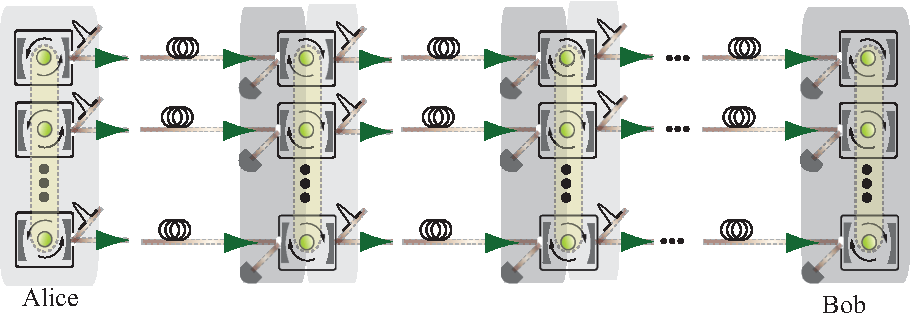
\includegraphics[width=\textwidth]{repeaters_9}
\caption{\comment{Redo fig}Schematic illustration of the transmission of a quantum signal using loss based error correction codes in a quantum network.}
\label{fig:repeaters_9}
\end{figure*}

The quantum state is then transferred/teleported via photons which are transmitted through a lossy channel to the adjacent repeater node. Here two specific operations occur: first the information encoded on each photon is transferred to a matter qubit within that repeater node and then that photon is measured. The photon measurement is critical as it heralds which photons have been lost and allows us to measure the remaining qubit in that block in the $\hat{X}$ basis, which removes the damaged parity blocks from our encoded state, leaving our information intact. We can now add the full redundancy back into our encoded state in the matter qubits. The fully encoded state can then be transferred to photons and transmitted to the next repeater node where the same procedure occurs again. This continues until our state reaches the last repeater node where Bob is.

There is one immediate observation that can be made from this scheme. The matter qubits (quantum memories) within the local nodes are only used to encode and error correct the redundancy code as well as transmitting those quantum states as photons. Entanglement is not stored within the nodes while the photons are being sent to the adjacent repeater nodes. This in turn means the resources within that repeater node can be used immediately again (once the photons have been transmitted), and so the rate of communication is now limited by the time to perform the local operations within a node, rather than the round trip time between adjacent nodes. 

The focus so far has been only on loss-based errors but this code is fault-tolerant to general errors as well \cite{bib:MKLLJ14}. Furthermore, this redundancy code was only an illustrative example that photon loss in the channel can be corrected. Many other codes can be used in a similar fashion \cite{bib:munro12, bib:Fowler10, bib:MKLLJ14}. Finally the scheme we have presented in Fig.~\ref{fig:repeaters_9} transmits a quantum signal from Alice and Bob. It can however be adapted to use the butterfly design from Fig.~\ref{fig:repeaters_8} to create remote entanglement between Alice and Bob while maintaining the performance advantages our direct transmission scheme gave. 

\subsection{Resource scalings across repeater generations}\index{Resource scaling}

As can seen the various quantum repeater generations take quite different approaches as to how they distribute entanglement between Alice and Bob over a long distance \cite{bib:Muralidharan2016}. It is useful thus to summarise in Table.~\ref{tab:rep_nets_scale} the performance of the various repeater approaches and their requirements.

\begin{widetext}
\begin{center}
\begin{table}[!htb]
\centering
\begin{tabular}{ccccc}
\hline
\multicolumn{1}{|l|}{\textbf{Repeater generation}} & \multicolumn{1}{l|}{\rm $T_\mathrm{av}$}   & \multicolumn{1}{l|}{\rm Resources consumed}    & \multicolumn{1}{l|}{\rm  $L_\mathrm{max}$}     & \multicolumn{1}{l|}{\rm  Local gate precision}     \\ \hline \hline
\multicolumn{1}{|l|}{First generation}    & \multicolumn{1}{l|}{$O(L_\mathrm{tot}/c)$} & \multicolumn{1}{l|}{$O(\mathrm{poly}(L_\mathrm{tot}))$} & \multicolumn{1}{l|}{\rm arbitrary}  & \multicolumn{1}{l|}{\rm arbitrary}    \\ \hline
\multicolumn{1}{|l|}{Second generation}   & \multicolumn{1}{l|}{$O(2 L/c)$}     & \multicolumn{1}{l|}{$O(\mathrm{polylog}(L_\mathrm{tot}))$} & \multicolumn{1}{l|}{\rm arbitrary}  & \multicolumn{1}{l|}{\rm high}   \\ \hline
\multicolumn{1}{|l|}{Third generation}   & \multicolumn{1}{l|}{$O(t_\mathrm{local})$}     & \multicolumn{1}{l|}{$O(\mathrm{polylog}(L_\mathrm{tot}))$} & \multicolumn{1}{l|}{$L/L_0<0.69$}   & \multicolumn{1}{l|}{\rm fault tolerant levels}   \\
\hline
\end{tabular}
\caption{Quantum repeater approaches and their expected performance scalings.  $T_\mathrm{av}$ corresponds to the time between which the protocol can be attempted (the time to generate a single Bell state is at least $L_\mathrm{tot}/c$) \cite{bib:Muralidharan2016}. The generation rate is $R\sim 1/T_\mathrm{av}$. Further given are the resources (quantum memories) required as well as the precision for the local gate operations within repeater nodes. $L_\mathrm{max}$ is the maximum spacing between repeater nodes. $L_\mathrm{tot}$ is the total distance between Alice and Bob while $L$ is the distance between adjacent repeater nodes. $t_\mathrm{local}$ is the time required to perform the local operations within the repeater node, while $L_0$ is the attenuation length of the channel/fibre.}
\label{tab:rep_nets_scale}
\end{table}
\end{center}
\end{widetext}

Table.~\ref{tab:rep_nets_scale} clearly shows that the average time to generate the Bell pair between the end nodes of the repeater network decreases significantly as we move to higher generation quantum repeaters. In the first generation our generation rate is $O(c/L_\mathrm{tot})$, which increases to $O(c/L)$ for the second generation schemes, and finally to $O(1/t_\mathrm{local})$ for the third generation ones. The difference here could be more than nine orders of magnitude. Next the number of quantum memories required decreases from $O(\mathrm{poly}(L_\mathrm{tot}))$ for the first generation approach to $O(\mathrm{polylog}(L_\mathrm{tot}))$ for the higher ones. The higher generation schemes however come at quite a cost, with the requirement for fully fault-tolerant (or near fault-tolerant) quantum gates within nodes. In fact, it's likely that Alice and Bob will have multiple potential routes between themselves.

\comment{Up to here}

\subsection{The transition to quantum networks}

The previous quantum repeater networks we discussed have been simple point-to-point\index{Point-to-point network} linear networks\index{Linear network}, as shown in Fig.~\ref{fig:repeaters_10}(a). While there were a number of ways to establish the end-to-end entangled links between Alice and Bob, they knew they were connected via a simple linear chain.
 
\begin{figure}[!htb]
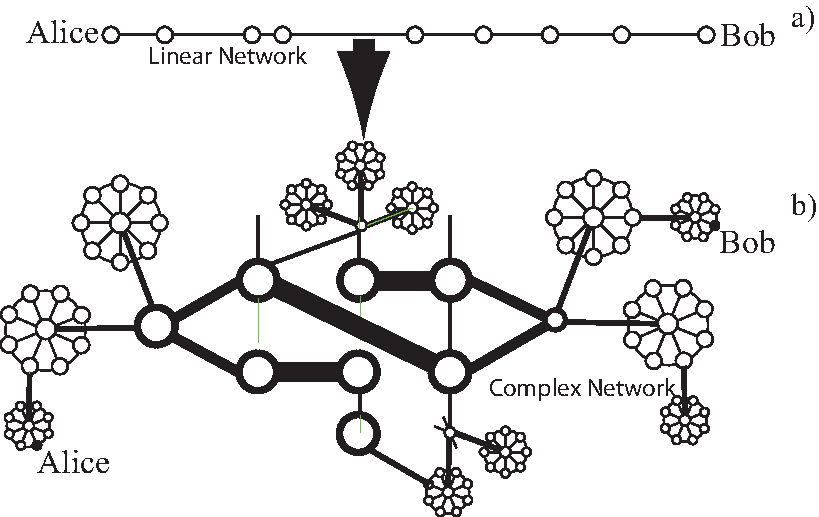
\includegraphics[width=0.475\textwidth]{repeaters_10}
\caption{\comment{Redo fig}Schematic illustration of two quantum network topologies. (a) The typical simple point-to-point linear quantum repeater network. (b) A network with a more complex (and realistic) topology, that could in principle support many simultaneous users. The thicker connecting lines indicates that links between nodes have more capacity.}
\label{fig:repeaters_10}
\end{figure} 

Of course this is highly unrealistic. Alice and Bob are likely to be members of a complex quantum network, e.g Fig.~\ref{fig10}(b), that supports multiple users simultaneously. This leads to a number of interesting considerations going forward. 

\begin{itemize}
\item For large-scale networks the users may not know its exact network topology or even the best route between them. In fact there could be multiple paths between Alice and Bob. Probing the entire network to establish the best route would be slow and costly (in practice). Still, every node should have a unique identifier (quantum IP address), uniquely indicating its location in the network.
\item Most complex networks dynamically change in time as resources become congested or nodes break. This in turn means using a butterfly approach to create Alice and Bob's links is problematic as one does not know the middle point between them to start the entanglement creation process. If one has to determine the route in advance and restrict access to those parts of the network required to establish the entire links, congestion will quickly follow. The generation rate will be very slow. 
\item Finally, it's unlikely that repeater nodes will be equally spatially separated (making the first generation repeater schemes extremely hard to use in this situation). 
\end{itemize}

The above issues lead us to a network model where Alice and Bob suspect there is a route between them but not the exact route, which is likely to be dynamic, i.e the availability of routes and their relative costs are liable to change. In such a case if Alice wants to send a message to Bob, she uses her knowledge of Bob's rough location (from the quantum IP address) and her knowledge of the nodes close to her to send a message to a repeater node who will have more knowledge of Bob's part of the network. This node can then forward the message to further nodes (who know even more about Bob's location) until it finally reaches Bob. The quantum IP address is essential here as that identifier indicates to the repeater node who to forward to next. In principle as the message (or entanglement) is being established node by node, those repeater nodes who have already been used are free to work for tasks for other users. 

There is another interesting aspect of our general complex quantum networks. There are likely to be many paths between Alice and Bob which could be attempted in superposition fashion. This will not only increase the capacity between Alice and Bob but also its robustness. 

\bibliography{bill}

\end{document}






%%%%%%%%%%%%%%%%%%%%%%%%%%%%%%%%%%%%%%



\bibitem{Nei00}  M. A. Nielsen and I. L. Chuang,  \textit{Quantum Computation and Quantum Information} (Cambridge Univ. Press, 2000).
%
\bibitem{Spiller2006}  T P Spiller and W J Munro, Towards a Quantum Information Technology Industry, J. Phys.: Condens. Matter {\bf 18}, V1-V10 (2006).
%
\bibitem{dowling02} J.P. Dowling, J. P. \& G.J. Milburn, Quantum technology: the second quantum revolution. Preprint at $<$http://arxiv.org/abs/quant-ph/0206091$>$ (2002).
%
\bibitem{Gisin2002}  N. Gisin, G. Ribordy, W.Tittel and H.  Zbinden, Quantum cryptography, Rev. Mod. Phys. {\bf 74}, 145-195 (2002).
%
\bibitem{Shor1997} P. W. Shor, Polynomial-time algorithms for prime factorization and discrete logarithms on a quantum computer SIAM J. Sci. Statist. Comput. {\bf 26}, 1484 (1997).
%
\bibitem{Feynman82} R. P. Feynman, Simulating Physics with Computers. Int. J. Theoret. Phys.  {\bf 21}, 467-488 (1982)
%
\bibitem{Caves1982} C. M. Caves, Quantum limits on noise in linear amplifiers, Phys. Rev. D {\bf 26}, 1817 (1982).
%
\bibitem{Giovannetti2004} V. Giovannetti, S. Lloyd, and L. Maccone,  Quantum-Enhanced Measurements: Beating the Standard Quantum Limit, Science {\bf 306}, 1330 (2004).
%
\bibitem{BB84} C. H. Bennett and G. Brassard,  \emph{Proceedings of IEEE International Conference on Computers, Systems, and Signal Processing}, Bangalore, India, IEEE Press (New York) 175-179 (1984).
%
\bibitem{Bennett96} C.H. Bennett, G. Brassard, S. Popescu, B. Schumacher, J. Smolin and W. K.  Wootters, Purification of Noisy Entanglement and Faithful Teleportation via Noisy Channels, Phys. Rev. Lett. {\bf 76}, 722 - 726 (1996).
%
%
\bibitem{Deutsch85} D. Deutsch, Quantum-theory, the Church-Turing Principle and the Universal Quantum Computer, Proc. R. Soc. Lond. A {\bf 400}, 97, 117 (1985).
%
\bibitem{lloyd96} S. Lloyd, Universal Quantum Simulators, Science {\bf 273}, 1073-1078 (1996).
%
\bibitem{Ladd2010} T.D. Ladd, F. Jelezko, R. Laflamme, Y. Nakamura, C. Monroe and J. L. O�Brien, Quantum computers, Nature {\bf 464}, 45�53 (2010).
%
\bibitem{commercial} See for instance http://www.idquantique.com/ , http://magiqtech.com,  http://quintessencelabs.com/, http://www.sequrenet.com
%
\bibitem{grover97} L. K. Grover, Quantum telecomputation. http://arXiv.org/quant-ph/9704012. (1997).
%
\bibitem{cirac99} J.I. Cirac, A. Ekert, S. Huelga and C. Macchiavello,  Distributed quantum computation over noisy channels. Phys. Rev. A {\bf 59}, 4249 (1999). 
%
\bibitem{meter2009} R. Van Meter, W. Munro, K. Nemoto and K. Itoh, Arithmetic on a distributed- memory quantum multicomputer, ACM Journal on Emerging Technologies in Computing Systems {\bf 3}, 2 (2009).
%
\bibitem{Darpa} Quantum cryptography network gets wireless link - info-tech - 7 June 2005 - New Scientist

\bibitem{Secoqc} M. Peev {\it et. al.}, New J. Phys. {\bf 11}(7), 075001/1-37 (2009).
%
\bibitem{TokyoQKD} M. Sasaki {\it et. al.}, Opt. Express {\bf 19}, 10387-10409 (2011).
%
\bibitem{Gerhardt2011} I. Gerhardt, Q. Liu, A. Lamas-Linares, J. Skaar, C. Kurtsiefer and V. Makarov, Full-field implementation of a perfect eavesdropper on a quantum cryptography system, Nature Communications {\bf 2}, 349 (2011).
%
\bibitem{bennett93}  C.H. Bennett, G. Brassard, C. Crepeau, R. Jozsa, A. Peres, and W.K. Wootters,  Teleporting an unknown quantum state via dual classical and Einstein-Podolsky-Rosen channels, Phys. Rev. Lett. {\bf 70}, 1895 (1993). 
%
\bibitem{cleve99}  R. Cleve, D. Gottesman, and H. Lo, How to Share a Quantum Secret, Phys. Rev. Lett. {\bf 83}, 648 (1999).
%

%
\bibitem{ekert91} A.K. Ekert, Quantum cryptography based on Bell's theorem, Phys. Rev. Lett. {\bf 67}, 661 (1991).
%
\bibitem{bbm92} C. H. Bennett, G. Brassard, and N. D. Mermin, Quantum cryptography without Bell's theorem, Phys.
Rev. Lett. {\bf 68}, 557 (1992).
%
\bibitem{SP00} P.W. Shor and J. Preskill, Simple proof of security of the BB84 quantum key distribution protocol, Phys.Rev. Lett. {\bf 85}, 441 (2000).
 %

%
\bibitem{chen07a} B. Zhao, Z.B. Chen, Y. A. Chen, J. Schmiedmayer and J. W. Pan, Robust creation of entanglement between remote memory qubits, Phys. Rev. Lett. {\bf 98}, 240502 (2007).
%
\bibitem{sheng08} Z. Yuan, Y. Chen, B. Zhao, S. Chen, J. Schmiedmayer and J. W. Pan, Experimental demonstration of a BDCZ quantum repeater node, Nature {\bf 454}, 1098-1101 (2008). 
%
\bibitem{simon07} C. Simon {\it et. al}, 
%C. Simon, H. de Riedmatten, M. Afzelius M, N. Sangouard, N. Zbinden and N. Gisin, 
Quantum Repeaters with Photon Pair Sources and Multimode Memories, Phys. Rev. Lett {\bf 98}, 190503 (2007).
%
\bibitem{sangouard09} N. Sangouard, R. Dubessy and C. Simon, Quantum repeaters based on single trapped ions, Phys. Rev. A {\bf 79}, 042340 (2009).
%

%
\bibitem{jiang09} L.~Jiang, J.M. Taylor, K.~Nemoto, W.J Munro, R. Van Meter, and M.D. Lukin, Quantum repeater with encoding, Phys.Rev. A {\bf 79}, 032325 (2009).
%
\bibitem{meter09}  R. Van Meter, T. D. Ladd, W. J. Munro and K. Nemoto, System Design for a Long-Line Quantum Repeater, IEEE/ACM Transactions on Networking {\bf 17}, 1002 (2009). 
%
\bibitem{munro10}
W. J. Munro, K. A. Harrison, A. M. Stephens, S. J. Devitt and K. Nemoto, From quantum multiplexing to high-performance quantum networking, Nature Photon. {\bf 4} , 792-796 (2010). 
%
\bibitem{Stute2013} A. Stute, B. Casabone, B. Brandst�tter, K. Friebe, T.E. Northup, and R. Blatt, Quantum-State Transfer from an Ion to a Photon, Nat. Photonics {\bf 7}, 219 (2013).
%
\bibitem{Volz2011} J. Volz, R. Gehr, G. Dubois, J. Est�ve, and J. Reichel, Measurement of the Internal State of a Single Atom without Energy Exchange, Nature (London) {\bf 475}, 210 (2011).
%
\bibitem{Greve2012} K. De Greve {\it et. al.}, 
% K. De Greve, L. Yu, P. L. McMahon, J. S. Pelc, C. M. Natarajan, N. Y. Kim, E. Abe, S. Maier, C. Schneider, M. Kamp, S. H�fling, R. H. Hadfieeld, A. Forchel, M. M. Fejer, and Y. Yamamoto, 
Quantum-Dot Spin-Photon Entangle- ment via Frequency Downconversion to Telecom Wave-length, Nature (London) 491, 421 (2012).
%
\bibitem{Gao2013}  W. B. Gao, P. Fallahi, E. Togan, J. Miguel-Sanchez, and A. Imamoglu, Observation of Entanglement between a  {Quantum} Dot Spin and a Single Photon, Nature (London) {\bf 491}, 426 (2012).
%
\bibitem{Schaibley2013} J. R. Schaibley {\it et.al}, 
%J. R. Schaibley, A. P. Burgers, G. A. McCracken, L. M. Duan, P. R. Berman, D. G. Steel, A. S. Bracker, D. Gammon, and L.J. Sham, 
Demonstration of Quantum Entanglement between a Single Electron Spin Confined to an InAs Quantum Dot and a Photon, Phys. Rev. Lett. {\bf 110}, 167401 (2013).
%
\bibitem{waks2006} E. Waks and J. Vuckovic, Dipole Induced Transparency in Drop-Filter Cavity-Waveguide Systems, Phys. Rev. Lett. {\bf 96}, 153601 (2006).
%
\bibitem{hu2008} C. Y. Hu, A. Young, J. L. OBrien, W. J. Munro, and J. G. Rarity, Giant Optical Faraday Rotation Induced by a Single-Electron Spin in a Quantum Dot: Applications to Entangling Remote Spins via a Single Photon, Phys. Rev. B {\bf 78}, 085307 (2008).
%
\bibitem {santori210} C. Santori, D. Fattal, and Y. Yamamoto, Single-Photon Devices and Applications (Wiley, New York, 2010).
%
\bibitem{nemoto2014} K. Nemoto {\it et .al}, 
%K. Nemoto, M. Trupke, S. J. Devitt, A. M. Stephens, B. Scharfenberger, K. Buczak, T. Nobauer, M. S. Everitt, J. Schmiedmayer, and W. J. Munro, 
Photonic Architecture for Scalable Quantum Information Processing in Diamond, Phys. Rev. X {\bf 4}, 031022 (2014).
%
\bibitem{Braunstein95} S. L. Braunstein and A. Mann, Phys. Rev. A {\bf 51}, R1727 (1995).
%
\bibitem{entangledpairs} C. Jones, K. De Greve and Y. Yamamoto, A high-speed optical link to entangle quantum dots, arXiv:1310.4609v1
%
\bibitem{Childress2005}  L. Childress, J. M. Taylor, A. S. Srensen, and M. D. Lukin, Fault-Tolerant Quantum Repeaters with Minimal Physical Resources and Implementations Based on Single-Photon Emitters, Phys. Rev. A 72, 052330 (2005).
%
\bibitem{munro12}  W.~J.~Munro, A.~M.~Stephens, S.~J.~Devitt, K.~A.~Harrison, K.~Nemoto, Quantum communication without the necessity
 of quantum memories, Nature Photon {\bf 6}, 777 (2012).
%
\bibitem{werner1989} Reinhard F. Werner, Quantum states with Einstein-Podolsky-Rosen correlations admitting a hidden-variable model, Physical Review A {\bf 40}, 4277�4281 (1989).



\bibitem{Stephens2013} Ashley M. Stephens, Jingjing Huang, Kae Nemoto, and William J. Munro, Hybrid-system approach to fault-tolerant quantum communication, Phys. Rev. A {\bf 87}, 052333 (2013).
%
\bibitem{Hartmann07} L. Hartmann, B. Kraus, H.-J. Briegel and  W. Dur, On the role of memory errors in quantum repeaters, Phys. Rev. A {\b 75}, 032310 (2007).
%
\bibitem{R09} M. Razavi, M.Piani and N. L\"utkenhaus, Quantum repeaters with imperfect memories: Cost and scalability, Phys.Rev. A {\bf 80}, 032301 (2009)
%
\bibitem{RB01} R. Raussendorf and H. J. Briegel, A one-way quantum computer, Phys. Rev. Lett.~{\bf 86}, 5188-5191 (2000).
%
\bibitem{K07} P Kok {\it et. al}, 
%P Kok, W. J. Munro, Kae Nemoto, T. C. Ralph, Jonathan P. Dowling, and G. J. Milburn, 
Linear optical quantum computing with photonic qubits, Rev. Mod. Phys.{\bf 79}, 135–174 (2007), and references therein.
%

\bibitem{D00} D. P. DiVincenzo, The physical implementation of quantum computation. Preprint at $\langle$http://arxiv.org/abs/quant-ph/0002077$\rangle$.
%
\bibitem{S10} C.~Simon {\em et al.}, Quantum memories. Eur. Phys. J. D {\bf 58}, 1-22 (2010).
%C. Simon, M. Afzelius, J. Appel, A. Boyer de la Giroday, S. J. Dewhurst, N. Gisin, C. Y. Hu, F. Jelezko, S. Kroll, J. H. Muller, J. Nunn, E. S. Polzik, J. G. Rarity, H. De Riedmatten, W. Rosenfeld,A. J. Shields, N. Skold, R. M. Stevenson, R. Thew,  I. A. Walmsley, M. C. Weber, H. Weinfurter, J. Wrachtrup and R. J. Young, Quantum memories. Eur. Phys. J. D {\bf 58}, 1-22 (2010).
%
\bibitem{Laflamme96} R. Laflamme, C. Miquel, J. Paz, and W. Zurek, quant-ph/9602019 (1996)
%
\bibitem{knill96} E. Knilland R. Laflamme, Theory of quantum error-correcting codes, Phys. Rev. A {\bf 55}, 900 (1997).

